\documentclass[licencjacka]{pracamgr}

\usepackage{polski}
\usepackage[utf8]{inputenc}
\usepackage{graphicx}
\usepackage{minted}
\usepackage{ltablex
\usepackage{tabularx}
\usepackage{pbox}

% Dane magistranta:

\autor{Michał Jaroń}{348711}
\autori{Jarosław Socha}{347267}
\autorii{Piotr Zalas}{361374}

\title{Framework oparty o wzorzec mikrousług na przykładzie portalu dla ZUS}

%\tytulang{Framework based on microservices pattern illustrated by portal for ZUS}

\kierunek{Informatyka}

% informatyka - nie okreslamy zakresu (opcja zakomentowana)
% \zakres{Tu wpisac, jesli trzeba, jedna z opcji podanych wyzej}

% Praca wykonana pod kierunkiem:
% (podać tytuł/stopień imię i nazwisko opiekuna
% Instytut
% ew. Wydział ew. Uczelnia (jeżeli nie MIM UW))
\opiekun{mgra Michała Możdżonka}

% miesiąc i~rok:
\date{Maj 2017}

%Podać dziedzinę wg klasyfikacji Socrates-Erasmus:
\dziedzina{ 
%11.0 Matematyka, Informatyka:\\ 
%11.1 Matematyka\\ 
%11.2 Statystyka\\ 
11.3 Informatyka\\ 
%11.4 Sztuczna inteligencja\\ 
%11.5 Nauki aktuarialne\\
%11.9 Inne nauki matematyczne i informatyczne
}

%Klasyfikacja tematyczna wedlug AMS (matematyka) lub ACM (informatyka)
\klasyfikacja{
	% \begin{CCSXML}
	%	<ccs2012>
	%	<concept>
	%	<concept_id>10011007.10011006.10011066.10011068</concept_id>
	%	<concept_desc>Software and its engineering~Software as a service orchestration system</concept_desc>
	%	<concept_significance>500</concept_significance>
	%	</concept>
	%	</ccs2012>
	%\end{CCSXML}
	%
	%\ccsdesc[500]{Software and its engineering~Software as a service orchestration system}
	Software and its engineering\\
	Software notations and tools\\
	Development frameworks and environments\\
	Software as a service orchestration system
	%Software and its engineering~Software as a service orchestration system
}

% Słowa kluczowe:
\keywords{Mikrousługi, Frontend, Backend, Integracja usług, Framework, Angular 2, Django, Python, TypeScript, ZooKeeper}

\begin{document}
\maketitle

%tu idzie streszczenie na strone poczatkowa
\begin{abstract}
	Praca przedstawia opis projektu i implementacji frameworka integracji mikrousług.
	Omawiamy typowe problemy występujące przy integrowaniu usług, sposoby ich
	rozwiązywania i zastosowane przez nas podejście z wykorzystaniem mikrousług.
	Prezentujemy przegląd już istniejących technologii oraz kryteria ich doboru
	do tworzonego przez nas rozwiązania. Następnie przedstawiamy architekturę i
	praktyczną realizację portalu do komunikacji między obywatelem a urzędem z
	wykorzystaniem opracowanego przez nas frameworka.
\end{abstract}

\tableofcontents
%\listoffigures
%\listoftables

%\chapter{Organizacja pracy}

%Pierwszym poważnym wyzwaniem, przed którym staneliśmy, była organizacja pracy zespołu. Każdy członek zespołu
%pochodzi z innego miasta i uczęszcza na inne zajęcia, ponadto część członków pracuje. Znalezienie pory i dnia
%tygodnia, w którym moglibyśmy się spotykać, stanowiło spore wyzwanie. W gospodarowaniu czasem i ustalaniu terminów
%spotkań z klientem bardzo nam pomogło doodle. % Mądrze rozwinąć!
%Komunikacja między członkami zespołu odbywała się głównie przez internet, przy pomocy facebooka %i slacka.
%Projekt prowadziliśmy w lekko zmodyfikowanej zwinnej metodyce opracowanej specjalnie na potrzeby naszego klienta.

\chapter{Wprowadzenie}\label{r:wstep}

\section{Motywacja}

Celem naszego projektu było stworzenie prototypu internetowego frameworka do komunikacji obywatela z urzędami
podobnego do Platformy Usług Elektronicznych ZUS \cite{zuspue}, a następnie zaimplementowanie na niej kilku wybranych przypadków użycia. Dzięki temu petent chcący
coś załatwić w urzędzie nie będzie musiał wychodzić z domu. Pewną inspiracją do stworzenia takiego systemu był
rządowy portal obywatel.gov.pl \cite{mcobywatel}.

Wyzwaniem, które należało uwzględnić w fazie projektowania, był szeroki zakres użytkowników systemu: od zwykłych
obywateli, poprzez urzędników, aż po przedsiębiorców. Każda z tych grup użytkowników miałaby zupełnie inne uprawnienia:
byłoby co najmniej niestosowne, gdyby przedsiębiorca wnioskowałby o urlop macierzyński dla prowadzonej przez siebie
firmy. Podobnie obywatel nie powinien mieć możliwości przyznania sobie emerytury lub renty (o ile nie jest urzędnikiem). Główne przypadki użycia systemu sprowadzałyby się do trzech wariantów: wypełniania wniosków, sprawdzania
odpowiedzi na wypełniony wniosek i rozpatrywania wniosków. Pobocznymi przypadkami byłyby: rezerwacja terminu wizyty w
urzędzie w przypadku nadzwyczaj zawiłych spraw, prezentacja różnych danych użytkownikowi (np. stanu ubezpieczenia,
wysokości przyznanej renty lub wymaganego ustawowo pouczenia) oraz wymiana korenspondencji z urzędnikiem. W obecnie
istniejącym systemie PUE jest jeszcze jeden przypadek użycia: czat z konsultantem. Nasza platforma powinna umożliwiać
stosunkowo prostą realizację niemal wszystkich spośród wymienionych wyżej przypadków użycia.

Kiedy użytkownik zaloguje się do naszego serwisu powinien zobaczyć pulpit, na którym wyświetlone są ,,kafelki''
odpowiadające poszczególnym usługom. Kliknięcie na wybrany kafelek powinno wyświetlić bardziej szczegółowy widok
odpowiadający podjętej akcji. Szczególnym życzeniem naszego klienta było, by architektura naszej aplikacji była
oparta na mikrousługach. Każda mikrousługa otrzymywałaby na wyłączność fragment pulpitu ograniczony do kafelka,
z możliwością przełączenia do trybu pełnoekranowego, gdzie przejmowałaby wtedy kontrolę nad większością wyświetlanego
obszaru. Aby to umożliwić, należało opracować ustandaryzowany i łatwo rozszerzalny interfejs do komunikacji między
cienkim klientem a mikrousługą. Preferowane było rozwiązanie, w którym komunikacja odbywałaby się bez pośrednictwa
serwera serwującego stronę internetową. Zamiast tego wykonywane byłyby asynchroniczne zapytania do mikrousługi (być
może poprzez warstwę integracji).

Postawione przed nami wymagania były głównie natury niefunkcjonalnej. Dołączanie kolejnej usługi do systemu
powinno być maksymalnie proste. Na tę prostotę składałby się ustandaryzowany interfejs do komunikacji pomiędzy
poszczególnymi usługami oraz modułowy i łatwo rozszerzalny interfejs użytkownika.
To pozwoli nam stosunkowo małym kosztem podłączać i odłączać kolejne usługi wraz z
rozwojem cyfrowej administracji. Usługi powinny tworzyć jeden ekosystem, z którego nie wychodziłby użytkownik. System
powinien być w dużej mierze odporny na awarie i zachowywać spójność oraz poprawność przechowywanych danych obywateli.
W szczególności powinny być spełnione normy ,,12 Factor App'' \cite{tfa}, w tym ta mówiąca, że awaria jednego serwera
lub usługi nie powinna wpływać na działanie pozostałych, niezależnych od niej udostępnianych usług.
Rozwój i utrzymanie platformy powinien być możliwy także dla mniej doświadczonych
programistów, których zatrudnienie generuje mniejsze koszty wytworzenia kodu. W ten sposób nasz projekt realizowałby plan
zrównoważonego rozwoju, zapobiegając centalizacji ośrodków programistycznych, a z drugiej strony prowadziłby do wymiernych
oszczędności na wynagrodzeniach.

\section{Pomysłodawca - ZUS}

Naszym zleceniodawcą był Zakład Ubezpieczeń Społecznych. Według ,,Rocznika
Statystycznego Ubezpieczeń Społecznych'' \cite{rocznik} w 2011 roku w ZUS było ubezpieczonych
14 milionów obywateli. Dochód Zakładu wyniósł w owym roku 155 796 milionów
złotych. Do obsługi takiej ilości petentów i zarządzania taką kwotą pieniędzy
było zatrudnionych przeciętnie 44 766 urzędników.

W związku z tym, że projektowaliśmy system dla administracji państwowej z
którego będą korzystać miliony obywateli, musieliśmy bardzo ostrożnie dobierać
technologie, z których korzystaliśmy. Wybranie rozwiązania opartego na
niekorzystnej licencji mogło się w przyszłości łączyć z problemami w postaci
konieczności zapłacenia bardzo wysokiej opłaty licencyjnej, wyłączenia usługi i
przebudowania jej na nowo, udostępnienia części systemu na licencji open source,
a nawet konieczności nieodpłatnego przekazania przechowywanych danych obywateli
licencjodawcy. Preferowane były rozwiązania, które albo były oparte na tzw. wolnych licencjach (Apache, MIT), albo takie, do
których nasz klient licencje już posiadał (m. in. IBM DB2, komercyjna wersja
PostgreSQL oraz korporacyjne rozwiązania firmy Microsoft). W miarę możliwości
powinniśmy korzystać z nowoczesnych, przyszłościowych i rozwijanych technologii,
tak, by odsunąć jak najdalej w przyszłość konieczność przebudowy systemu z
powodu zmieniających się trendów i narastającego długu technologicznego.

Innym istotnym aspektem naszego projektu było zerwanie z wizerunkiem ZUSu jako
instytucji przestarzałej, niewydolnej i przeciążonej biurokracją. Szata graficzna naszej platformy powinna być przyjemna dla oka, a układ
graficzny elementów logiczny, prosty do zrozumienia i konsekwentny. Użytkownik
nie może być bombardowany zagadkowo brzmiącymi komunikatami o ,,wchodzeniu na
poziom bezpieczeństwa 1'' i ,,zamiarze korzystania z usług biznesowych'', a sytuacje takie miały nierzadko miejsce w obecnej, produkcyjnej wersji platformy PUE. 
W żadnym przypadku praca z naszym systemem nie powinna przypominać nieprzyjemnych interakcji, jakich można doświadczyć w tzw. urzędowym "okienku", a to
nakłada na nas obowiązek rozwiązania problemu skalowalności aplikacji.

\section{Produkt końcowy}

Nasz produkt spełnia wymienione wyżej oczekiwania. Dzięki zastosowaniu nowoczesnej
architektury frameworka zapewniona została wysoka skalowalność, niezawodność oraz
łatwość i wygoda użycia. Udowodniliśmy te stwierdzenia poprzez implementację przykładowego
portalu realizującego wybrane przez naszego Klienta reprezentatywne przypadki użycia.
Całość została podana w przyjaznej dla oka oprawie. Uważamy, że z powodu wymienionych
wyżej czynników można uznać nasz projekt za zakończony sukcesem.

\chapter{Wymagania}

Głównym wymaganiem postawionym przed naszym frameworkiem było umożliwienie reimplementacji
Platformy Usług Elektronicznych ZUS \cite{zuspue} (widocznej na poniższym obrazku) oraz stworzenie
przykładowego portalu ilustrującego jego możliwości.\\
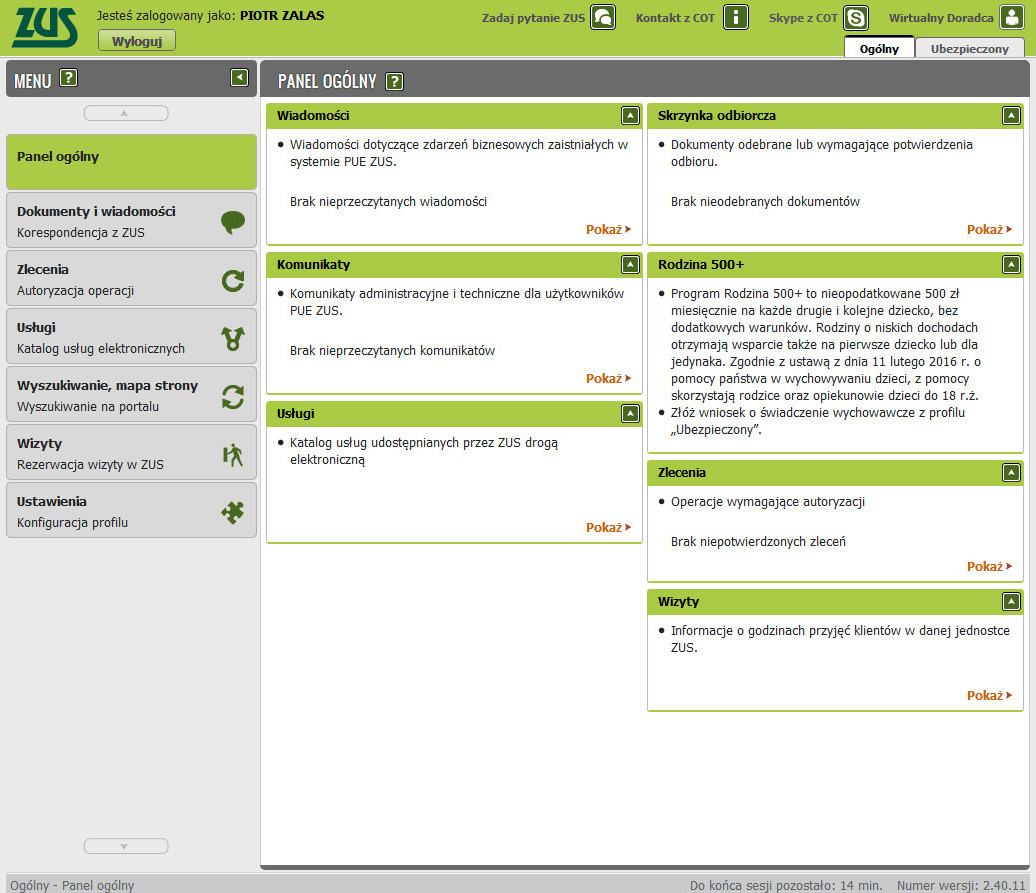
\includegraphics[width=\textwidth]{obrazki/pue2.png}
Naszemu zespołowi pozostawiono bardzo duży stopień swobody przy projektowaniu i
implementacji portalu. Główny nacisk położono na innowacyjność stworzonego rozwiązania.
Niezależnie od tego, w trakcie naszych rozmów z Klientem zostały wyłonione przedstawione
niżej wymagania.

\section{Wymagania funkcjonalne}

Stworzony przez nas portal powinien implementować kilka rezprezentatywnych
przypadków użycia celem ilustracji możliwości naszego frameworka i łatwości,
z jaką się w nim tworzy aplikacje. Wybraliśmy następujące przypadki użycia:
powiadomienia, skrzynkę pocztową, usługę 500 plus.

Najprostrzym w implementacji przypadkiem użycia jest sprawdzanie dostępnych
powiadomień przez użytkownika. Tuż po udanym wejściu na nasz portal użytkownikowi
powinien zostać wyświetlony ekran na którym zobaczyłby krótkie statystyki i
informację, co zmieniło się od jego ostatniej wizyty na portalu.

Kolejna grupa przypadków użycia związana jest z mechanizmem przypominającym
wewnętrzną pocztę. Użytkownik powinien być w stanie wyświetlić listę wysłanych
i odebranych wiadomości. Po wybraniu odpowiedniej wiadomości z listy powinna
ukazać mu się jej treść. Możliwa jest też odpowiedź na wiadomość do nadawcy.
Szczególnie istotny jest fakt, że z opisanego mechanizmu mogą korzystać różne
usługi. Przykładowo, usługa odpowiedzialna za obsługę wniosków 500+ wysyła
wiadomości związane z różnymi zdarzeniami dotyczącymi cyklu życia wniosku.

Sztandarowym przypadkiem użycia ilustrującym pełnię możliwości naszego frameworka
jest usługa odpowiedzialna za wnioski 500+. Użytkownik może przy jej pomocy
wypełnić i złożyć wniosek o świadczenie. Po wysłaniu formularza powinien otrzymać
stosowne powiadomienie na swoją skrzynkę pocztową. Następnie będzie mógł sprawdzić
status złożonego wniosku oraz podejrzeć jego treść. W międzyczasie urzędnik ZUS
otrzyma dostęp do panelu, w którym będzie mógł zdecydować o dalszych losach
wniosku. Jeżeli po sprawdzeniu załączonych danych postanowi zaakceptować lub
odrzucić wniosek, to będzie mógł to uczynić przy pomocy odpowiedniego guzika.
Informacja o tym fakcie natychmiast zostanie doręczona do wnioskodawcy.

\section{Wymagania niefunkcjonalne}

Bardzo wiele uwagi poświęciliśmy wymaganiom niefunkcjonalnym. Nasz Klient bardzo
wyraźnie życzył sobie, by spełnione były normy ,,12 Factor App'' \cite{tfa}.
Niektóre spośród nich są stosunkowo proste: kod powinien być trzymany w systemie
kontroli wersji, należy bardzo wyraźnie określać zależności, konfiguracja pobierana
jest z środowiska, powinno być możliwe bezbolesne przeniesienie usług wspomagających
(takich jak bazy danych) do zewnętrznych dostawców (np. chmury AWS). Pozostałe
normy odnoszą się do takich zagadnień jak zapewnienie jednolitości środowisk testowych
i produkcyjnych, wykorzystanie dobrodziejstw płynących z współbieżności oraz
zarządzanie już działającą aplikacją. Z naszego punktu widzenia najważniejsza była
następująca zasada: nasz serwis powinien cechować się wysokim współczynnikiem
niezawodności i odporności na losowe awarie. Ma to szczególne duże znaczenie
podczas komunikacji na linii obywatel -- państwo, gdzie jakiekolwiek rozbieżności
mogą być opłakane w skutkach. W miarę postępu cyfryzacji państwa liczba użytkowników
naszego serwisu będzie zbliżać się do 14-tu milionów osób. Należy zapewnić
skalowalność tworzonej aplikacji w sposób pozwalający na ich obsłużenie.

Nasz serwis powinien cechować się spójnym i jednolitym wyglądem oraz wysoką
reużywalnością komponentów wykorzystywanych do tworzenia interfejsu użytkownika.
Interfejsy powininny być łatwo rozszerzalne bez łamania wstecznej kompatybilności
i konieczności modyfikacji już napisanych fragmentów aplikacji. W projekcie
należy uwzględnić dynamicznie zmieniające się środowisko w jakim przyjdzie działać
naszej aplikacji. Z powodu ciągle postępującej cyfryzacji państwa i związanych z
tym znacznych zmian w prawie możemy być pewni, że po oddaniu serwisu do użytku
ulegnie on znaczącym przekształceniom. Powinniśmy sprawić, by koszt owego przekształcenia
był jak najmniej dotkliwy dla naszego Klienta.

Wymaganiem bardzo podobnym do powyższego jest konieczność łatwej integracji z już
istniejącymi systemami informatycznymi. Przykładem takiego systemu w ZUS jest
,,Kompleksowy System Informatyczny''. Systemy które nie znajdują się pod zarządem ZUS
to między innymi ,,Profil Zaufany (eGO)'' oraz ,,System Rejestrów Państwowych''.
Nasz serwis powinien łatwo integrować się z wymienionym wyżej oprogramowaniem.
Należy uwzględnić fakt, że możliwość modyfikacji i dostosowania zewnętrznych
systemów do naszych potrzeb jest bardzo ograniczona.

Platforma powinna być prosta w użyciu nawet dla relatywnie nisko wykwalifikowanych
programistów i utrudniać im popełnienie przynajmniej części błędów. Przykład
problemu występującego w obecnej wersji PUE jest widoczny na poniższym obrazku.
Ze względu na niewłaściwą architekturę systemu możliwe jest wyświetlenie
użytkownikowi sprzecznych komunikatów dotyczących stanu zalogowania. Nasz framework
nie powinien pozwalać na powstanie takiej sytuacji.\\
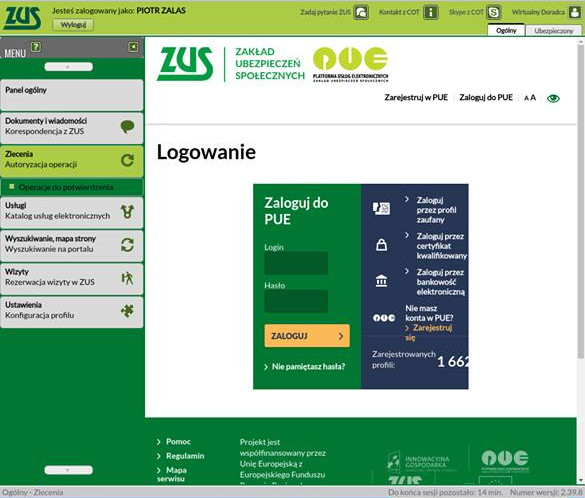
\includegraphics[width=\textwidth]{obrazki/logowaniezle.png}

System utworzony na bazie naszego frameworka powinien cechować się znacznym stopniem
automatyzacji. Dołączanie i odłączanie kolejnych serwerów powinno odbywać się w locie,
bez konieczności ręcznej rekonfiguracji. Ten postulat bardzo wydatnie łączy się z
wymaganiem skalowalności i niezawodności. Przeprowadzane zmiany w konfiguracji serwerów
nie powinny rzutować na niezawodność serwisu.

\chapter{Teoretyka}

\section{Problem}

Nasz produkt powinien w sposób maksymalnie prosty umożliwiać integrację systemów
informatycznych zakładu ubezpieczeń społecznych. Podstawowymi problemami jakie
należało uwzględnić na etapie projektowania systemu były:
\begin{itemize}
	\item Znaczny poziom skomplikowania istniejącego oprogramowania
	\item Duża ilość użytkowników naszego systemu
	\item Zapewnienie wysokiego poziomu odporności na awarie
\end{itemize}
Po przejrzeniu istniejących rozwiązań zaproponowaliśmy naszemu klientowi
architekturę opartą o mikrousługi.

\section{Mikrousługi}

Mikrousługi \cite{fowlermicroservices} to stosunkowo nowy wzorzec architektoniczny będący rozwinięciem
architektury zorientowanej na usługi (ang. \textit{service-oriented architecture}).
Cechuje się ona rozbiciem poszczególnych składowych systemu na małe, luźno powiązane
usługi implementujące logikę biznesową. Znacząco ułatwia to ciągłą integrację (ang.
\textit{continuous integration}) oraz wdrożenie (ang. \textit{deployment}) dużych,
bardzo złożonych aplikacji. Ponadto pozwala to na stosunkowo dużą różnorodność
wykorzystanych technologii i stopniową ewolucję wykorzystywanego stosu technologicznego
\cite{microsvc}.

Zastosowanie mikrousług upraszcza proces skalowania całego systemu, co ma niebagatelne
znaczenie dla naszego klienta. W systemach o architekturze monolitycznej skalowanie
odbywa się na dwa sposoby: poprzez zastosowanie mocniejszej jednostki obliczeniowej
lub przez uruchomienie kolejnej instancji aplikacji na nowym serwerze. Pierwsze
podejście ma tę wadę, że stosunkowo szybko można osiągnąć górny pułap wydolności
dostępnego na rynku sprzętu. W drugim przypadku niezbędne jest zapewnienie mechanizmów
synchronizacji i replikacji danych, co w bardzo rozbudowanych systemach może okazać się
praktycznie niewykonalne. Architektura mikrousług oferuje mitygacje wymienionych problemów,
gdyż dzięki rozbiciu systemu na wiele małych usług możliwe jest
wystawienie każdej usługi na osobnym serwerze, zaś luźne ich powiązanie pomaga
zredukować nakłady na synchronizację pomiędzy poszczególnymi mikrousługami, dzięki
czemu kod staje się prostszy w utrzymaniu i modernizacji.

Zazwyczaj uznaje się, że każda mikrousługa powinna mieć własną bazę danych \cite{nginx},
do której pozostałe usługi nie mają bezpośredniego dostępu. Dzięki temu łatwiejsze
staje się wymuszenie luźnego powiązania usług, a ewolucja schematu bazy danych nie
wymusza zmian w całym kodzie aplikacji. Ponadto zespół pracujący nad daną mikrousługą
może w sposób nie wpływający na pozostałą część systemu wybrać tę bazę danych, która
najbardziej odpowiada rozwiązywanemu problemowi.

Niestety architektura zorientowana na mikrousługi ma swoje wady \cite{hauer}.
Do najpoważniejszych należy konieczność utrzymywania spójności danych w niezależnych
od siebie systemach bazodanowych. Ze względu na rozproszoną naturę aplikacji
wiele operacji wymaga interakcji z kilkoma niezależnymi od siebie serwerami baz
danych. Może się okazać, że z powodu awarii łączy pomiędzy serwerami część
transakcji nie zostanie wykonana co doprowadzi do rozspójnienia danych. W systemach
administracji publicznej nie powinno dochodzić do takich sytuacji, gdyż może to
doprowadzić do realnych i niezawinionych szkód u obywatela. Innymi problemami
nierozłącznie związanymi z mikrousługami są: mniej wygodny interfejs programisty
w porównaniu z architekturą monolityczną, konieczność uwzględniania w projekcie
aplikacji problemów występujących w warstwie sieciowej (takich jak awarie sprzętu
sieciowego) oraz niższa wydajność z powodu latencji przy przesyłaniu danych przez
sieć oraz konieczności serializacji i deserializacji zapytań.

Niezależnie od tych wad uważamy, że w naszej aplikacji zastosowanie architektury
mikrousługowej jest całkowicie racjonalnym rozwiązaniem. Zalety mikrousług w dużej
mierze rekompensują wymienione wyżej wady.

\section{Bezstanowość mikrousług}

Wśród dobrych praktyk konstruowania oprogramowania opartego o mikrousługi \cite{nginx}
jest ta, mówiąca o traktowaniu serwerów w sposób bezstanowy. Poszczególne serwery
należy traktować jak wymienialnych członków grupy. Wszystkie pełnią te same role i
wykonują tę samą pracę. Jeżeli jeden z nich ulegnie awarii, to obowiązki uszkodzonej
maszyny mogą przejąć pozostałe instacje. Podobnie dostawienie kolejnej instancji
nie powinno sprawiać większych trudności. Dzięki temu uzyskujemy teoretycznie
nieograniczoną skalowalność.

\section{Integracja mikrousług}
W naszej architekturze mikrousług potrzebowaliśmy jakiejś metody komunikacji
pomiędzy poszczególnymi mikrousługami. Poniżej wypisaliśmy najczęściej spotykane
rozwiązania tego problemu.

\subsection{Szyny danych}

Na początku nasza uwaga została przykuta przez szyny danych jako standardowe rozwiązanie korporacyjne wykorzystywane
przy integracji usług. Nasz klient jest w posiadaniu licencji na szynę danych WebMethods i to ją jako pierwszą
rozpatrywaliśmy. Niestety, dostępna publicznie internetowa dokumentacja tego rozwiązania ograniczała się do kilku
broszurek reklamowych i luźnych sloganów. Z czystej ostrożności zrezygnowaliśmy z tego oprogramowania, gdyż nie
mieliśmy absolutnie żadnej gwarancji, że wyczytane hasła reklamowe mają jakiekolwiek pokrycie w rzeczywistości.
Do kolejnej grupy sprawdzonych szyn danych należały rozwiązania takie jak: WSO2, Talend, Mule. Możliwości, które
oferowały wyglądały na obiecujące, ale zupełnie niepasujące do specyfiki naszego projektu. Jednym z celów naszej
platformy było opracowanie interfejsu, który pozwalałby na możliwie łatwe, automatyczne wpinanie i wypinanie
mikrousług. Nijak do tak postawionego celu miała się konieczność konfigurowania szyny danych przez panel wystawiony w sieci
WWW lub wręcz przy pomocy specjalnego środowiska programistycznego takiego jak Eclipse, z obowiązkową fazą kompilacji
i wgrywania na serwer. 

Rozwiązaniem wartym wspomnienia jest Zato, dość osobliwa szyna danych rozwijana przez osobę o polsko brzmiącym nazwisku. Jej głównymi cechami są skalowalność, możliwość rekonfiguracji w locie oraz bardzo dobra integracja z językiem python, co miało dla nas niebagatelne znaczenie na etapie wczesnych analiz. W zasadzie cała logika realizowana przez tę szynę danych mogła być zapisana w postaci skryptu pythona, co otwierało nas na zupełnie nowe możliwości integracji mikrousług. Rozważaliśmy scenariusz, w którym szyna danych odpowiadałaby za wykrywanie działających mikrousług, trzymanie ich spisu i metadanych z nimi powiązanych oraz rozgłaszanie tegoż spisu do warstwy prezentacji i innych mikrousług. Zrezygnowaliśmy z tego podejścia jako naruszającego zasadę separacji odpowiedzialności.

\subsection{Kolejki komunikatów}
Niepowodzenia przy poszukiwaniu odpowiadającej nam szyny danych skierowały nas w kierunku innych rozwiązań, takich jak
kolejki komunikatów. Głównym wymaganiem jakie postawiliśmy była bardzo duża odporność na różnego rodzaju błędy i
awarie. W idealnym modelu każda wiadomość w kolejce powinna mieć trzy stany: do przetworzenia, w trakcie przetwarzania, wykonany. Celem takiego modelu jest, by w przypadku awarii jednego serwera usługi jego zadanie było transparentnie przekazane serwerowi zastępczemu, bez przerywania operacji. Udało nam się znaleźć tylko jedną kolejkę spełniającą to wymaganie - Beanstalkd \cite{beanstalkd}.

Innym sposobem osiągnięcia niezawodności może być kolejka ukryta wewnątrz mikrousługi, która w razie awarii jednego serwera pozwalałaby na odczytanie zadania przez inny serwer i dokończenie go. Niestety wtedy mogą mieć miejsce problemy z atomowością operacji. Przykładowo, w sytuacji gdy zadanie w kolejce zostało oznaczone jako wykonane, ale usługa wywołująca nie otrzymała jeszcze odpowiedzi nastąpi awaria wywoływanej mikrousługi, może dojść do duplikacji wykonanej operacji lub rozspójnienia danych.

\subsection{Dzienniki}

Jeszcze innym, ciekawym podejściem byłoby zastosowanie usługi udostępniającej niezawodny dostęp do czegoś w rodzaju dziennika. Wtedy moglibyśmy stosunkowo małym kosztem zaimplementować mechanizmy stosujące transakcyjność rodem z relacyjnych baz danych. Przykładami takich usług są DistributedLog \cite{distibutedlog} i Kafka \cite{kafka}. Poszczególne mikrousługi monitorowałyby dziennik i z niego pobierały zmiany, a następnie reagowały na nie poprzez podjęcie jakiejś akcji. Można sobie wyobrazić dwa sposoby wykorzystania takiego dziennika. Pierwszy polegałby na tym, że wszystkie dokonane zmiany są atomowo publikowane w jednej dużej paczce, która musiałaby być potem rozpakowywana, a poszczególne zmiany wyłuskiwane. Drugim sposobem byłoby stworzenie dużej ilości dzienników na każdy rodzaj zdarzenia, a każda operacja byłaby wykonywana w małych krokach, w sposób potokowy.

\subsection{Rozwiązania oparte o BPMN}
W wymienionych wyżej modelach komunikacji serwery pośredniczące w wymianie
komunikatów nic nie wiedzą o procesach biznesowych, w których uczestniczą. 
Możliwa jest jednak realizacja zgoła przeciwnego podejścia, w którym działanie
wszystkich mikrousług jest koordynowane przez jedną centralną usługę.

Pozwalala ona na modelowanie procesów biznesowych przy pomocy graficznej
,,Notacji i Modelu Procesu Biznesowego'' (ang. \textit{Business Process Modeling
Notation}), a następnie wykonanie ich na specjalnie do tego celu skonstruowanym
silniku. Poszczególne mikrousługi stanowią w tym modelu ,,klocki'', z których
klient może sobie kontruować bardziej złożone procesy. Przykładami technologii,
które implementują wyżej wymienioną funkcjonalność są:
\begin{itemize}
	\item Camunda (oparty na Activiti)
	\item Bonita BPM
	\item jBPM
	\item Intalio BPMS
\end{itemize}

James Lewis i Martin Fowler w swojej publikacji \cite{fowlermicroservices}
stwierdzają, że powyższe podejście nie jest preferowane w środowisku mikrousług
gdyż stanowi złamanie zasady ,,sprytnych końcówek i bezmyślnych łączy'' (ang.
\textit{smart endpoints and dumb pipes}).

\section{Problemy z współbieżnością mikrousług}

Nietrudno wyobrazić sobie sytuację, w której dwie współbieżnie działające mikrousługi
wprowadzają konfliktujące ze sobą zmiany. Pewną formą zabezpieczenia przed takimi sytuacjami
mogłoby być rozwiązywanie konfliktów przez mikrousługę pośredniczącą w dostępie do bazy danych.
Taka mikrousługa stanowiłaby wtedy coś w rodzaju sekcji krytycznej, uniemożliwiającej jednoczesne zapisy
i niespójne odczyty (niezależnie od atomowości operacji na bazie danych). 
Niestety, takie podejście może nie wystarczać, np. w przypadku dwóch niezależnie działających usług, które wpierw
odczytują jakąś informację z bazy danych, a następnie na podstawie uzyskanej informacji wybierają rodzaj
akcji do podjęcia i nadpisują część bazy danych.

Jest kilka możliwych rozwiązań tego problemu. Możemy je pogrupować ze względu na następujące cechy:
\begin{itemize}
	\item miejsce przechowywania blokad
	\item sposób zakładania blokad na usługi
	\item wielkość obiektów, które będą blokowane
\end{itemize}
Blokady mogą być przechowywane w dedykowanej, wydzielonej mikrousłudze lub w mikrousłudze, której dotyczą. W naszej opinii
pierwsze podejście jest o tyle lepsze, że pozwala na wykrywanie zakleszczeń. Wadą takiego rozwiązania jest
stosunkowo słabe zrównoleglanie i fakt, że taka mikrousługa stanowiłaby najsłabszy punkt systemu, którego awaria
skutkowałaby zablokowaniem wszystkich pozostałych usług. Blokady mogą być zakładane pojedyńczo, w miarę
postępu transakcji lub na jej samym początku (w takim przypadku mikrousługa musi dokładnie wiedzieć, z jakich
zasobów ma zamiar skorzystać). Wydaje nam się, że najsensowniejszym wariantem jest wykorzystanie rozwiązań
stosowanych w relacyjnych bazach danych, gdzie blokady są zakładane w miarę postępu transakcji, a w przypadku
wykrycia zakleszczenia zmiany są wycofywane, sama zaś usługa wywłaszczana. Przy kolejnej próbie takiej mikrousłudze
nadany zostaje większy priorytet, który zapewnia żywotność. W przypadku implementacji takiego podejścia należy
pamiętać o zapewnieniu mechanizmów wywłaszczania mikrousług, księgowania zmian, śledzenia transakcji, wykrywania
zakleszczeń, nadawania priorytetów oraz o możliwości zakładania możliwie małych blokad na pojedyńcze rekordy.

Innym sposobem rozwiązania wyżej przedstawionego problemu jest zakładanie blokad na początku transakcji.
Ze względów wydajnościowych blokowanie przez muteks
całych mikrousług zapewniających dostęp do danych nie jest możliwe. Z uwagi na opóźnienia w przesyłaniu informacji
przez sieć prowadziłoby to z jednej strony do marnowania mocy obliczeniowej serwera bazy danych, a z drugiej strony
znacząco ograniczałoby ilość jednoczesnych operacji. Z kolei zakładanie blokad na konkretne wiersze w poszczególnych
mikrousługach jest nierealizowalne, gdyż w chwili zakładania muteksu usługa może nie wiedzieć, jakie konkretnie
wiersze zmodyfikuje. Uznaliśmy, że złotym środkiem jest zakładanie blokady na właściciela danych. Wynika to z
faktu, że w typowej urzędniczej praktyce wykonywane operacje dotyczą co najwyżej kilku osób.

Uzbrojeni w powyższe informacje wytypowaliśmy dwie usługi mogące działać jako zarządca rozproszonego muteksa:
redisson \cite{redisson} i ZooKeeper \cite{zookeeper}. Redisson jest rozwiązaniem implementującym algorytm Redlock
\cite{redislock}. Jego najważniejszą cechą jest odporność na awarie usług poprzez automatyczne zwalnianie blokady
po upływie określonego czasu. W internecie ukazała się bardzo interesująca polemika do przytoczonego algorytmu \cite{redisbad}.
Głównym zarzutem czynionym wobec algorytmu Redlock jest brak mechanizmu, który zapobiegałby następującej sytuacji:
mikrousługa A zakłada blokadę na zasób Z. Następnie zaczyna operację nadpisywania danych. W trakcie operacji
działanie mikrousługi z losowego powodu zostaje zawieszone (np. wystąpiło znaczne opóźnienie w połączeniu sieciowym
lub włączył się odśmiecacz pamięci). W tym czasie termin ważności blokady mija, zostaje ona zdjęta, a do akcji
wkracza mikrousługa B, która zakłada swoją blokadę, nadpisuje dane utworzone przez usługę A i kończy swoje
działanie. Na koniec usługa A zostaje wybudzona i kontynuuje swoje działanie, prowadząc do rozspójnienia danych.
Według autora polemiki rozwiązaniem tego problemu jest skorzystanie z mechanizmu współdzielonej blokady
zaimplementowanej w frameworku Apache Curator \cite{curatorlock} i korzystającej pod spodem z Apache ZooKeepera.
Jest to bezpieczniejsze rozwiązanie które nie pozwala na wygaśnięcie blokady z powodu upływającego
czasu, a w przypadku awarii mikrousługi i utraty połączenia z nią
automatycznie zdejmuje blokadę. Ponadto, jest to stosunkowo nowoczesny projekt wykorzystywany i rozwijany przez
duże firmy takie jak Netflix, co daje pewne nadzieje dotyczące stabilności i dojrzałości tego projektu.

\section{Rejestracja i wykrywanie mikrousług}

Zarządzanie infrastrukturą w systemie opartym o mikrousługi jest znacznie większym
wyzwaniem niż w systemie o architekturze monolitycznej. Dzieje się tak z powodu
dużej ilości różnych serwerów usług a także dlatego, że mikrousługi zachęcają do
stosowania wielu różnorodnych, nierzadko niekompatybilnych technologii. Ręczna
konfiguracja i administrowanie takim systemem pochłania znaczne zasoby, dlatego
postanowiliśmy ten proces zautomatyzować. Przedstawimy kilka powszechnie stosowanych
w przemyśle rozwiązań tego problemu.

Pierwszym z nich jest serwer Apache ZooKeeper \cite{zookeeper}. Dane na serwerze
ZooKeeper są trzymane w drzewiastej strukturze. Każdy węzeł może zawierać dowolny
ciąg bajtów ograniczony do rozmiaru ok. 1 Mb. Serwer pozwala na atomowe odczyty i
zapisy, ponadto może działać w klastrze. W takim przypadku gwarantowane jest zachowanie
sekwencji zapisów. Dostęp do danych jest chroniony przez mechanizm ACL.
Informacje o mikrousługach są przechowywane w węzłach drzewa i zazwyczaj składają
się na nie identyfikator serwera, adres internetowy, port usługi, informacja o
obsłudze SSL. Dzięki otwartości kodu źródłowego klient usługi dostępny jest na
większości wiodących platform.

Rozwiązaniem bardzo podobnym do ZooKeepera jest Consul. Zasadniczą różnicą
między tymi dwoma serwerami było zastosowanie w Consulu słownika typu
klucz-wartość oraz znacznie bardziej zaawansowane raportowanie stanu
mikrousługi, które obejmuje nie tylko informację o działaniu serwera usługi,
ale także okresowe sprawdzanie jego stanu przy pomocy specjalnie
zaprojektowanego RESTowego interfejsu. Ułatwia on integrację z platformami na
których nie jest dostępny klient Consula. Consul jest projektem komercyjnym.

Podobną, chociaż nieco okrojoną funkcjonalność w stosunku do Consula zapełniają
serwery etcd i Netflix Eureka. Ten pierwszy pozwalał na rozproszone składowanie
danych w słowniku typu klucz-wartość. Eureka z kolei zapewniała automatyczną
rejestrację, wykrywanie i odpytywanie mikrousług z zadaną częstotliwością oraz
monitorowanie ich stanu. Obydwa projekty mają otwarty kod źródłowy.

\section{Wnioski}

Nasz zespół zdecydował, że opracujemy rozwiązanie wykorzystujące mikrousługi.
Komunikacja z poszczególnymi serwerami powinna być bezstanowa. Konfiguracja
mikrousług będzie przechowywana w formie drzewa w centralnym serwerze o dużym
stopniu niezawodności.

Rozwiązania realizujące komunikację między mikrousługami uważamy za wysoce
niewystarczające i zbyt mało elastyczne. Postanowiliśmy stworzyć własną usługę
o funkcjonalnościach zbliżonych do szyny danych, która na dodatek pozwala na
zautomatyzowaną konfigurację bez przerywania swojej pracy.

Nasz framework nie będzie rozwiązywał problemu rozproszonej synchronizacji między
usługami. Wynika to z bardzo dużej różnorodności sposobów na jakie można to uczynić.
Nasza platforma może integrować poprzez różne adaptery już istniejące usługi,
które zupełnie nie są świadome istnienia zaproponowanego mechanizmu blokad,
więc możliwe byłyby niekompatybilności między rozwiązaniem zaproponowanym
przez nas a wymienionymi usługami. Przykładami problematycznych usług mogą być
,,System Rejestrów Państwowych'' oraz ,,Kompleksowy System Informatyczny'' do
których dokumentacji z oczywistych względów nie mamy dostępu, więc nie możemy
przewidzieć trudności jakie nasza platforma będzie narzucać naszym użytkownikom.
To programiści korzystający z naszego systemu będą musieli rozwiązać ten problem
w sposób, jaki uznają za optymalny.

\chapter{Wykorzystane technologie}

Nasz serwis wykorzystuje bardzo dużą ilość różnych technologii. Związane jest to
z charakterem naszego projektu, który polegał na integracji usług napisanych w
możliwie różnych technologiach.

\section{Języki programowania}


Do napisania części backendowej początkowo wykorzystywaliśmy język Java. Głównymi
argumentami przemawiającymi za tym wyborem był bogaty zbiór bibliotek wykorzystywanych
w aplikacjach korporacyjnych, wysoka wydajność maszyny wirtualnej Java oraz fakt, że
obecnie istniejące systemy prawdopodobnie wykorzystują ten język. W trakcie naszych
prac okazało się, że jest to zupełnie nietrafiony wybór. Narastające problemy
pojawiające się podczas współpracy z wybranymi bibliotekami oraz niezadowalające
tempo prac w połączeniu ze zbliżającymi się terminami skłoniły nas do przepisania
już napisanego oprogramowania na język Python.

W przypadku naszego projektu radykalna decyzja o zmianie wykorzystywanego ekosystemu
była o tyle prosta, że nasz serwis miał charakter prototypu ilustrującego pewne
idee i niewykorzystywanego w środowisku produkcyjnym. Bardzo szybko okazało się, że
była to trafiona decyzja pozwalająca na mitygacje problemów, które pojawiły się w
trakcie naszych prac.

\section{Angular 2}

Aby rozwinąć swoje skrzydła, asynchroniczne działanie mikrousług wymaga również działającej asynchronicznie warstwy użytkownika.
Spośród obecnie stosowanych frameworków frontendowych wyróżniały się dwa: Angular \cite{angular2} oraz React.js \cite{react}.
Zdecydowaliśmy się na ten pierwszy z powodu kluczowej dla klienta, całkowicie otwartej licencji.
Licencja frameworka React.js była dla naszego klienta całkowicie nieakceptowalna
z powodu niejasnych zapisów, które dawały firmie Facebook prawo do cofnięcia zgody
na wykorzystanie frameworka \cite{reactlicense}. W przypadku instytucji państwowej
jaką jest ZUS było to obarczone niedopuszczalnym ryzykiem.
Wykorzystaliśmy drugą (w chwili wybierania technologii najnowszą) wersję Angulara
od Google. Wykorzystuje on język TypeScript, czyli obiektowe rozszerzenie języka Javascript.
W stosunku do JavaScript można stwierdzić, że wszystko co związane z obiektowością
w TypeScript to tylko lukier syntaktyczny, ponieważ kod TypeScript podczas kompilacji
jest tłumaczony do czystego JavaScript. TypeScript implementuje większość
funkcjonalności, które język obiektowy powinien oferować - możliwe jest dziedziczenie,
tworzenie interfesjów, konstruktory itp. Ciekawą opcją są dekoratory (szerzej opisane
w dalszej części pracy), czyli ozdobniki klas które pozwalają na zmianę ``zachowania''
klasy już w trakcie kompilacji.

\section{Bootstrap}

Za wygląd strony odpowiada HTML5, połączony z Bootstrapem \cite{bootstrap}.
Bootstrap to zbiór gotowych komponentów wizualnych, pozwalający, bez zbędnego wnikania
w stronę ,,artystyczną'', tworzyć strony estetyczne oraz wygodne w użyciu strony internetowe.
Jako, że tematem naszej pracy nie jest projektowanie stron internetowych i nie chcieliśmy zbytnio wnikać w aspekty graficzne,
użyliśmy gotowej skórki sbAdmin2, w której wprowadziliśmy liczne zmiany.

\section{Django}

Powszechnie przyjętym zwyczajem jest, że mikrousługi komunikują się przy pomocy
RESTowych API \cite{mammatustech}. Naszym zdaniem do kontrukcji takiego interfejsu
idealnie nadają się frameworki do tworzenia aplikacji webowych. Z uwagi na swoją
prostotę wybraliśmy Django \cite{django}. Dodatkowym argumentem za takim wyborem był tutaj fakt,
że architektura mikrousług zachęca do dywersyfikacji technologii. Wybierając
framework napisany w języku Python chcieliśmy pokazać, że nasze rozwiązanie dobrze
integruje usługi napisane w różnych językach.

\section{Express.js}

Do serwowania części frontendowej serwisu wykorzystujemy serwer Express.js \cite{expressjs}.
Korzystanie z niego jest proste i stosunkowo przyjemne, znakomicie integruje się
on z platformą Node.js. W przeciwieństwie do Lite--servera z którego korzystaliśmy
na początku, Express.js jest dobrze udokumentowany i udostępnia bogate API, z którego
skorzystaliśmy przy integracji z backendem.

\section{gRPC}

Podczas projektowania mechanizmu komunikacji pomiędzy mikrousługami nasz Klient
zasugerował użycie WSDL \cite{wsdl}. Nie zgodziliśmy się na to, gdyż użycie tak ciężkiego
protokołu jest sprzeczne z typowymi praktykami stosowanymi w architekturze
mikrousług \cite{mammatustech}. Jednocześnie nie chcieliśmy, by nasza aplikacja
była ograniczona tylko i wyłącznie do RESTowych protokołów. Ostatecznie
zaproponowaliśmy użycie gRPC \cite{grpc}, który łączy zalety obu wymienionych wcześniej
rozwiązań. Z jednej strony jest stosunkowo lekkim i wykorzystującym niewiele
zasobów protokołem sieciowym, a z drugiej strony pozwala na ścisłe zdefiniowanie
udostępnianych przez serwer usług w czytelnym dla ludzi formacie. Po napisaniu
odpowiednich definicji możliwa jest ich kompilacja do gotowego kodu źródłowego
włączanego bezpośrednio w pliki projektu. Dzięki temu minimalizowane jest ryzyko
popełnienia błędu przy pisaniu modułu do komunikacji z innymi usługami. Co ważne,
kompilator gRPC jest dostępny dla wszystkich wykorzystanych przez nas języków
programowania.

\section{Play Framework}

Play Framework \cite{play} opiera się na podobnych ideach architektonicznych co Django. Kiedy
go wybieraliśmy mieliśmy nadzieję, że będzie się on bardzo dobrze integrował z
ekosystemem Javowym. Okazało się, że było to błędne założenie. Kłopoty pojawiły
się już na samym początku, kiedy odkryliśmy że między frameworkiem Play i gRPC ma
miejsce konflikt zależności. Zdecydowaliśmy się użyć wersji niestabilnej, w
której ten konflikt był już rozwiązany. Narastające w trakcie trwania projektu
problemy ostatecznie zmusiły nas do porzucenia tego frameworka na rzecz Django.

\section{SQLite}

W naszym projekcie rodzaj użytej bazy danych nie miał większego znaczenia, gdyż
dostęp do niej odbywa się poprzez wyspecjalizowaną usługę zapewniającą dostęp do
danych lub w ramach jednej mikrousługi, gdzie służy jako tymczasowe składowisko
informacji potrzebnych przy wykonywaniu operacji. W takim modelu rodzaj użytej
bazy danych jest transparentny dla usługi wywołującej. Z uwagi na prototypowy
charakter naszego projektu poprzestaliśmy na bazie SQLite \cite{sqlite}, jako że znakomicie
integruje się ona z Django, ponadto zastąpienie jej PostgreSQLem \cite{postgres} jest
praktycznie bezkosztowe.

\section{ZooKeeper}

Jednym z elementów wizji naszego systemu był fakt, że poszczególne usługi
powinny możliwie prosto ,,wpinać się'' w system. Serwer mikrousługi w trakcie
uruchamiania dopisywałby do globalnej konfiguracji wpisy związane z prowadzoną
przez siebie działalnością, takie jak adresy pod którymi przyjmuje zapytania
albo pozycje w menu widocznym dla użytkownika, które prowadzą do poszczególnych
usług biznesowych. Doszliśmy do wniosku, że nasze oczekiwania można sprowadzić
do trzech wymagań:
\begin{itemize}
	\item przechowywania konfiguracji w drzewiastej strukturze
	\item automatycznego usuwania dokładnie określonych wpisów w przypadku
	utraty dowolnego serwera mikrousługi
	\item automatyczną replikację danych
\end{itemize}

Najbliższy naszym potrzebom był serwer Apache ZooKeeper \cite{zookeeper} w
połączeniu z biblioteką Apache Curator \cite{curator}. Dane na serwerze
ZooKeeper są trzymane w drzewiastej strukturze. Każdy węzeł może zawierać dowolny
ciąg bajtów ograniczony do rozmiaru ok. 1 Mb. Węzły są wersjonowane, a dostęp
do nich jest kontrolowany przez mechanizm ACL. Na każdym węźle można ustawić
obserwatora (ang. \textit{watch}), który w przypadku jakiejkolwiek modyfikacji
węzła powiadamia klienta o zmianie. Oprócz tego, każdy węzeł może mieć ustawione
dwie dodatkowe flagi. Pierwsza to \textit{ephemeral}, która oznacza, że węzeł ma
istnieć tylko do czasu zakończenia sesji klienta, który utworzył dany węzeł.
Ta własność jest szczególnie interesująca w kontekście automatycznego
wyrejestrowywania usługi która kończy swe działanie i nie ma możliwości
powiadomienia serwera o tym fakcie. Druga flaga to \textit{sequence}. Mówi ona,
że należy do nazwy tworzonego węzła dopisać rosnący numer. Ma to zastosowanie we
wszelkiego rodzaju kolejkach, algorytmach synchronizujących i przy wyborze
lidera \cite{curatorlock}.

\subsection{Curator}

Biblioteka Curator \cite{curator} upraszcza wiele aspektów związanych
z wykorzystaniem ZooKeepera, między innymi rejestrację serwerów mikrousług,
zapewnia implementację najczęściej wykorzystywanych algorytmów synchronizujących
oraz łatwe buforowanie drzewa węzłów wraz z automatycznym pobieraniem zmian. W
trakcie prac nad integratorem okazało się, że oferowane możliwości znacznie przekraczają
nasze potrzeby.

\subsection{Kazoo}

Kazoo \cite{kazoo} jest nieoficjalnym klientem ZooKeepera dla języka Python. W trakcie
implementacji naszej aplikacji doceniliśmy jego niezawodność i prostotę użycia.

\chapter{Architektura aplikacji}

Nasza aplikacja jest podzielona na trzy warstwy: frontend, mikrousługi oraz
warstwę integrującą, na którą składają się serwery autoryzacji i integratora.
Komunikacja pomiędzy poszczególnymi warstwami jest bezstanowa, co przynajmniej
w teorii powinno pozwolić na osiągnięcie niemal nieograniczonej skalowalności.

\section{Frontend}

Główną ideą którą kierowaliśmy się przy projektowaniu frontendu było udostępnienie
programiście mikrousług komponentów, z których mógłby następnie tworzyć interfejs
użytkownika. Jednym z wymagań zamawiającego było uczynienie tworzenie mikrosusług prostym,
stworzenie zestawu gotwoych komponentów, z których, jak z klocków, programista może
składać swój projekt, niewątpliwie upraszcza proces tworzenia nowych funkcjonalności.

Rzeczony opis utrzymany jest na wysokim poziomie abstracji --
jest w nim zawarta informacja \textbf{co} ma być wyświetlone, ale nie \textbf{jak}.
Użytkownik wchodzący na nasz portal poprzez przeglądarkę internetową otrzymuje
JSONa opisującego komponenty do wyświetlenia, który następnie jest przekonwertowany
na kod HTML dostosowany do jego przeglądarki. Dzięki temu, że wygląd panelu użytkownika
jest zapisany w formacie pośrednim możliwa jest zmiana wyglądu portalu bez
konieczności ponownego wdrażania wszystkich serwerów mikrousług.
Systemy służące do automatycznego
zarządzania pracownikami mogą zupełnie pomijać warstwę prezentacji i operować
bezpośrednio na danych dostarczanych przez warstwę integracji. 

\section{Warstwa integracji}

Kluczowym elementem tej warstwy jest integrator, przez który przechodzi niemal
cały ruch w systemie. Każda mikrousługa wchodząca w skład portalu musi być
zarejestrowana w integratorze. Dostęp do mikrousług jest możliwy tylko poprzez
integratora, który sprawdza, czy klient mikrousługi ma odpowiednie uprawnienia
dostępowe, dokonuje tłumaczenia komunikatów pomiędzy różnymi interfejsami,
wyszukuje adres serwera, do którego ma trafić komunikat oraz go wywołuje.

Z uwagi na to, że integrator ma wgląd w przechodzące przez niego dane, można
go podłączyć do ,,Systemu Wykrywania Intruzów'' (ang. \textit{Intrusion Detection System}) wykrywającego
anomalie w przesyłanych danych i w ten sposób zapobiegać masowemu wyciekowi
wrażliwych danych lub atakom hakerskim. Stanowi też dodatkową linię obrony, którą
musi sforsować potencjalny haker. Dzięki temu system jest odporniejszy na błędy
popełnione w serwerach mikrousług, a w przypadku wykrycia jakiejś luki można
wprowadzić łatkę bezpieczeństwa w serwerze pośredniczącym zamiast łatać
wszystkie podatne serwery mikrousług.

Integrator współpracuje z serwerem uwierzytelniania i autoryzacji, który przechowuje
listę wszystkich użytkowników systemu wraz z ich uprawnieniami. Dostęp do tego
serwera jest możliwy z dowolnej części sieci. Z uwagi na konieczność zapewnienia
łatwej integracji z zewnętrznymi usługami typu ,,Profil Zaufany (eGO)'', do
identyfikacji użytkowników użyliśmy jednorazowych tokenów.

\section{Mikrousługi}

Mikrousługi realizują logikę biznesową. Typowym cyklem życia serwera usługi jest
przygotowanie do obsługi nadchodzących żądań, rejestracja w integratorze i obsługa
zapytań. W końcowej fazie cyklu serwer się wyrejestrowuje z integratora. Realizacja
integratora oczekuje, że poszczególne serwery będą z punktu widzenia klienta
nierozróżnialne.

\section{Komunikacja między warstwami}

Z uwagi na stosunkowo duży poziom złożoności architektury naszej aplikacji opis
komunikacji podzieliliśmy na dwie części: backend i frontend. W obydwu dodatkowo
zawarliśmy warstwę integracji.

W części frontendowej (zaprezentowanej na poniższym obrazku) główną rolę odgrywa
serwer express.js, który serwuje do
przeglądarki na komputerze użytkownika kod aplikacji napisany w frameworku Angular.
Następnie otrzymany program zostaje wykonany, a użytkownikowi zostaje zaprezentowany
wygodny interfejs i możliwa staje się dalsza interakcja.

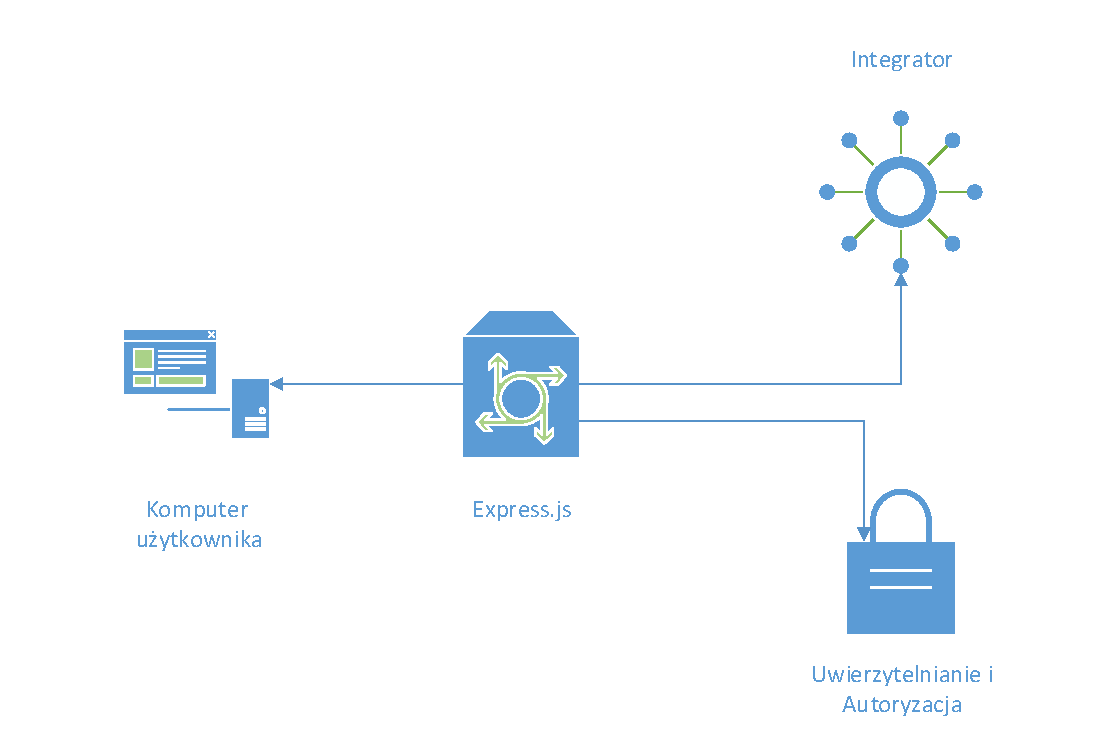
\includegraphics[width=\textwidth]{Frontend.pdf}

Z powodu różnych zabezpieczeń wbudowanych w przeglądarki bezpośrednie połączenie
klienta z integratorem nie jest możliwe. W związku z tym serwer express.js pełni
dodatkowo rolę pośrednika pomiędzy aplikacją internetową a integratorem i serwerem
autoryzacji. Pozostałe rodzaje klientów naszego portalu mogą go całkowicie pominąć.

Jak widać na poniższym schemacie, centralnym elementem w komunikacji elementów
backendu jest integrator. Przechodzi przez niego praktycznie cały ruch między
poszczególnymi mikrousługami i serwerami frontendu. Wyjątek stanowią tutaj serwery
ZooKeepera oraz uwierzytelniania, do których dostęp jest bezpośredni. Wynika to ze
specyficznych własności ZooKeepera który jest wykorzystywany do przechowywania
konfiguracji integratora oraz pewnego rodzaju wyjątkowości serwera autoryzacji,
która nie pozwala na zaklasyfikowanie go jako zwykłej mikrousługi.\\
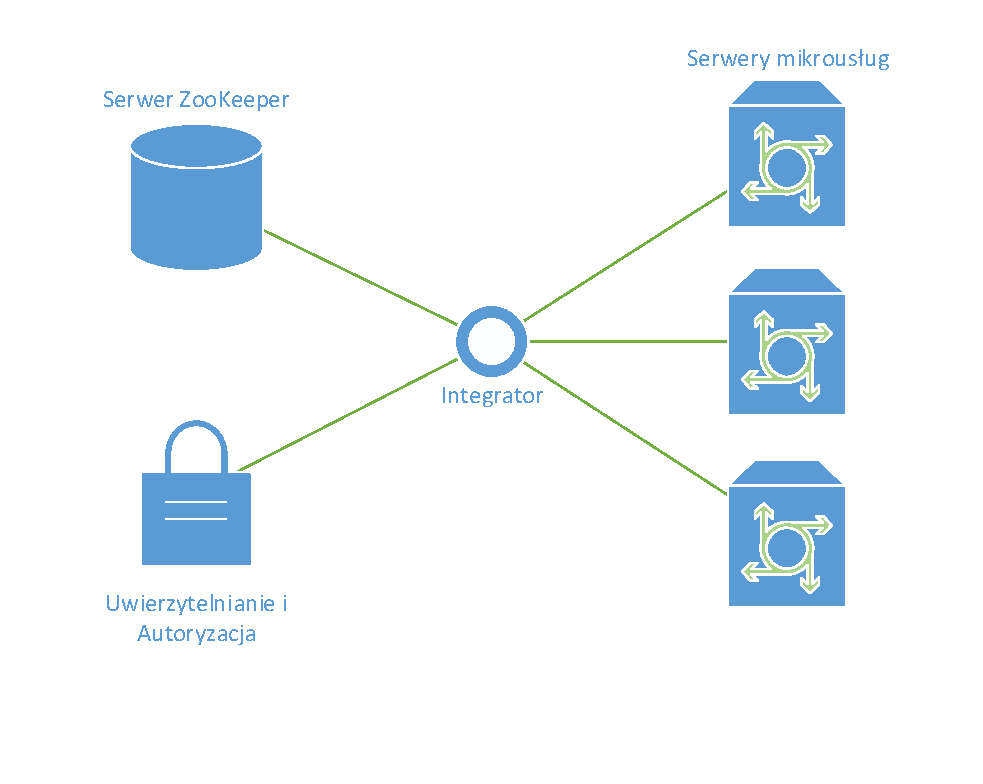
\includegraphics[width=\textwidth]{backend.pdf}

\chapter{Realizacja}

\section{Tworzenie mockupów}
Jako, że naszym celem nie było stworzenie gotowej platformy (w sensie produkcyjnym), a raczej stworzenie proof of concept,
dlatego intensywnie tworzyliśmy prototypy. Chcieliśmy pokazać, jak PUE może wyglądać, nie skupiając się jednak na
sprawach żmudnych, czasochłonnych i niekoniecznie potrzebnych do pokazanie idei (takich jak kwestie bezpieczeństwa - oczywiście
tego tematu całkowicie nie pominieliśmy - ale zapewnienie bezpieczeństwa dla takiego typu platformy nie było naszym głównym celem).

\section{Strona domowa}
Nastawienie społeczeństwa do ZUS, jako organizacji jest zdecydowanie negatywne, dlatego tworząc nasz projekt staraliśmy się
zmienić wizerunek ZUSu. Postawiliśmy na personalizacje kontaktów z użytkownikiem odwiedzającym naszą platformę. Dlatego już po zalogowaniu
użytkownik otrzymuje większość potrzebnych informacji. Strona domowa jest dopracowana pod względem UX. Panele informują
obywatela o aktualnym stanie spraw z nim związanych. Informację te są wyraźnie wyróżnione, a kolory jakie przyjmują panele
intuicyjnie wiążą się z kontekstem (np. czerwony kolor - sprawy odrzucone). Właściciel profilu nie musi marnować czasu
na szukanie najbardziej potrzebnych mu informacji, w innych miejscach strony. W założeniu, strona domowa powinna być
namiastką ,,Ściany'' znanej z popularnego portalu społecznościowego. Panel z powiadomieniami to po prostu dostarczony
przez nas gotowy komponent o nazwie powiadomienia. Po skasowaniu wszystkich aktualnych powiadomień wyświetla się spersonalizowany
komunikat, chwalący użytkownika za aktywność. To kolejny element wpisujący się w naszą filozofię tworzenia platformy jako
środowiska nie tylko użytecznego ale i przyjaznego.

\section{Komponenty}
\subsection{Mechanizm komponentów}

Projektując naszą platformę, pamiętaliśmy o istotnym nacisku, jaki klient kładł na jej proste rozszerzanie.
Postanowiliśmy zatem zaprojektować własny mechanizm, który usprawniłby wytwarzanie mikrousług gotowych do pracy w naszym systemie.
Od strony backendu dużo łatwiej jest uzgodnić wspólny interfejs, którego implementacja w nowej mikrousłudze pozwoli podłączyć ją do działającej platformy.
Frontend natomiast jest wytwarzany w zasadzie wyłącznie w języku HTML, ze wsparciem ze strony języka skryptowego Javascript oraz jego bibliotek.
Docelowe mikrousługi wykorzystywane na naszej platformie będą komunikowały się z REST-owym backendem.
Formularze z kolei posiadają zazwyczaj dosyć generyczne interfejsy graficzne i programistyczne.
Stając przed tak ocenioną sytuacją, postanowiliśmy nie oddawać w ręce programistów mikrousług możliwości umieszczenia na stronie platformy dowolnego kodu HTML.
Przede wszystkim ze względów bezpieczeństwa - usługa mogłaby uruchamiać zlośliwy bądź posiadający krytyczne luki kod javascript.
Ważne dla nas były jednak także kwestie stylistyczne - dużo wygodniej, niż publikować przewodniki styli (tzw. ,,Style Guide''),
byłoby nam udostępnić już gotowe, wystylizowane przez nas kawałki kodu HTML.

Osadzanie wewnątrz naszej aplikacji przekazanego w jakiś sposób szablonu HTML nie jest trudne, ale pozostaje pytanie o to,
na kim będzie spoczywała odpowiedzialność jego napisania. Nie chcieliśmy
żeby była do tego potrzebna wiedza frontendowa,
dlatego postanowiliśmy zwiększyć poziom abstrakcji w naszych szablonach,
a co za tym idzie -- zbudować mały framework (szkielet),
który uprości ich tworzenie, przekazywanie i interpretację, z poziomu osoby lub programu czytającego ich opis.

Uważamy, że większość elementów na stronach składająych się na aplikacje webowe można stworzyć składając mały zbiór gotowych elementów.
To właśnie dlatego wprowadzamy w naszym frameworku pojęcie komponentu. Komponenty to niepodzielne (patrząć z zewnątrz) części oferujące
pewien rodzaj aktywności. Sama ``definicja'' komponentów brzmi bardzo podobnie jak mikrousług, komponenty operują jednak w warstwie frontend,
to one korzystają z mirkousług, łączać logikę w jeden spójny klocek.

\subsection{Opis komponentów}

Każdy komponent oferuje pewien rodzaj aktywności, żeby lepiej pokazać różnicę między komponentem, a mikrousługą,
można posłużyc się metaforą. Stół do ruletki to jeden komponent składający się z komponentów, plansza, koła.
Komponent oferuję możliwość zagrania w ruletkę. Za losowanie(ruch kulki w kole) odpowiada już jednak mikroułsuga, za werfyfikacje
graczy również odpowiada mikrousługa. Z poziomu programisty używającego naszego komponentu nie widać jednak
tych poszczególnych części składowych. Programista chce w pewnym miejscy osadzić stół z ruletką, wklei więc w swój kod
<ruletka></ruletka>. Komponent stworzony już przez kogoś innego. Reużywalność kodu w najlepszej postacii.
Każdy komponent powinien posiadać unikalny w skali całego obiektu JSON identyfikator, ustawiany jako wartość pola $id$.
Jako, że pomimo różnych zadań zewnętrzny iterfejs komponentów jest w miarę podobny, 
poniżej znajduje się w miarę szczegółowy opis kilku wybranych komponentów: \\

\begin{tabularx}{\linewidth}{|l|l|c|X|l|}\hline
\textbf{Nazwa:}
Powiadomienie
\\\hline
\textbf{Opis:}\\

Rodzaj krótkiej wiadomości, składającej się z tytyłu i treści powiadomienia.\\\hline
\textbf{Końcówki:}\\
Końcówka pobierająca powiadomienie\\\hline
\textbf{JSON:}\\
\textit{title:} tytuł wiadomości\\
\textit{msg:} treść wiadomości, która zostanie rozwinięta w chwili kliknięcia na tytuł\\
\textit{time:} czas wysłania powiadomienia\\\hline
\textbf{Opis działania:}\\
Powiadomienie zostaje jednorazowo pobrane z podanej końcówki.\\\hline
\end{tabularx}

\begin{tabularx}{\linewidth}{|X|}\hline
\textbf{Nazwa:}
Lista powiadomień
\\\hline
\textbf{Opis:}\\

Pojemnik na powiadomienia, koordynujący pobieranie powiadomień\\\hline
\textbf{Końcówki:}\\
Końcówka z powiadomieniami\\
Końcówka z liczbą powiadomień(musi wiedzieć ile ściągnąć)
\\\hline
\textbf{JSON:}\\
\textit{title:}\\
\textit{msg:}\\
\textit{time:} \\ \hline
\textbf{Opis działania:}\\
Cyklicznie (w ustalonych odstępach czasu, obecnie co 5 sekund), komponent
wysyła zapytanie o liczbę dostępnych powiadomień, następnie w pętli, iteruje zwróconą liczbę razy,
pobierając za każdym razem powiadomienie z końcówki. Pobieranie powiadomienia z końcówki sprowadza się
do stworzenia komponentu Powiadomienia z danym adresem końcówki, a następnie osadzenie komponentu w sobie.\\\hline
\end{tabularx}

%\vspace{30pt}

\begin{tabularx}{\linewidth}{|X|}\hline
\textbf{Nazwa:}
PanelComponent
\\\hline
\textbf{Opis:}\\
Kontener z paskiem tytułowym i zawartością.\\
\hline
\textbf{Pola obiektu JSON:} \\
$title$: tytuł panelu\\
$panel\_class$: typ - kolor - panelu, wg. typów obsługiwanych przez bootstrap\\
$collapsible$: czy ciało panelu rozwijane\\
$hidable$: czy panel usuwalny\\
$backgroundColor$: kolor tła w ciele panelu\\
$textColor$: kolor tekstu w panelu\\
$cursor$: typ kursora (myszy) na obszarze panelu\\
$size$: obiekt o polach $xsmall, small, medium, large, xlarge$, opisujący dla jakiego rozmiaru okna, jak szeroki ma być panel w skali $0 - 12$ (mechanizm zapożyczony z bootstrapa)
\\\hline
\textbf{Opis działania:}\\
Komponent pozwalający obramować grupę innych komponentów w tak zwany panel.
W ciele panelu możliwe jest osadzanie innych komponentów. Panel może posiadać pasek tytułowy, oraz możliwość rozwijania\\\hline

\end{tabularx}

\begin{tabularx}{\linewidth}{|X|}\hline
\textbf{Nazwa:}
TextBox
\\\hline
\textbf{Opis:}\\

Pole tekstowe do wprowadzania danych\\
\hline
\textbf{Pola obiektu JSON:} \\
$defaultText$: tekst-wskazówka, tzw. placeholder\\
$text$: tekst domyślny, początkowa wartość\\
$regex$: wyrażenie regularne w składni javascript, do walidacji wprowadzonych danych\\
$visible$: czy komponent widzialny\\
Inne pola, np. $size$, jak w PanelComponencie wyżej
\\\hline
\textbf{Opis działania:}\\
Pole tekstowe czeka na dane od użytkownika. Przy pomyślnej walidacji, podświetla się na zielono, w przeciwnym wypadku na czerwono.
\\\hline
\end{tabularx}

\begin{tabularx}{\linewidth}{|X|}\hline
\textbf{Nazwa:}
PeselComponent
\\\hline
\textbf{Opis:}\\

Pole tekstowe do wprowadzania numeru PESEL\\
\hline
\textbf{Pola obiektu JSON:} \\
Jak w TextBox
\\\hline
\textbf{Opis działania:}\\
Pole tekstowe dostosowane domyślnie przez wyrażenie regularne do rozpoznawania liczb identyfikujących numer PESEL.
Dodatkowo w algorytmie walidacji jest liczona suma kontrolna PESELu.
\\\hline
\end{tabularx}

%\vspace{60pt}

\begin{tabularx}{\linewidth}{|X|}\hline
\textbf{Nazwa:}
ZipcodeComponent
\\\hline
\textbf{Opis:}\\

Pole tekstowe do wprowadzania kodu pocztowego\\
\hline
\textbf{Pola obiektu JSON:} \\
Jak w TextBox
\\\hline
\textbf{Opis działania:}\\
Pole tekstowe dostosowane domyślnie przez wyrażenie regularne do rozpoznawania kodów pocztowych formatu $00-000$
\\\hline
\end{tabularx}

\begin{tabularx}{\linewidth}{|X|}\hline
\textbf{Nazwa:}
FormComponent
\\\hline
\textbf{Opis:}\\

Formularz wysyłający swoją zawartość na podaną końcówkę\\
\hline
\textbf{Pola obiektu JSON:} \\
$form\_action$: adres URL końcówki, na którą zostanie wysłany formularz\\
$method$: metoda $get$ lub $post$ wysyłania zapytania na końcówkę\\
\hline
\textbf{Opis działania:}\\
Formularz wysyła na zadaną końcówkę zapytanie HTTP zawierające w treści zawartość pól, które są w nim osadzone.
\\\hline
\end{tabularx}

\begin{tabularx}{\linewidth}{|X|}\hline
\textbf{Nazwa:}
LabelComponent
\\\hline
\textbf{Opis:}\\

Etykieta - niemodyfikowalne pole tekstowe\\
\hline
\textbf{Pola obiektu JSON:} \\
$text$: treść wyświetlanego tekstu\\
$backgroundColor$: kolor tła etykietki\\
\hline
\textbf{Opis działania:}\\
Etykietka służy do wyświetlania tekstu dowolnej długości. Tekst jest zawijany, aby uniknąć konieczności przewijania strony w poziomie.
\\\hline
\end{tabularx}

\begin{tabularx}{\linewidth}{|X|}\hline
\textbf{Nazwa:}
DynamicListComponent
\\\hline
\textbf{Opis:}\\

Komponent, który pozwala użytkownikowi na replikację swojego komponentu potomnego dowolną liczbę razy\\
\hline
\textbf{Pola obiektu JSON:} \\
$replicableElement$: dowolny, pojedynczy komponent, który ma być replikowany\\
\hline
\textbf{Opis działania:}\\
Komponent potomny może być replikowany dowolną liczbę razy. Liczba kopii jest regulowana za pomocą przycisków $+/-$ zlokalizowanych u dołu komponentu. Domyślnie potomek jest jeden.
\\\hline
\end{tabularx}

%\vspace{60pt}

\begin{tabularx}{\linewidth}{|l|}\hline
\textbf{Nazwa:}
RowComponent
\\\hline
\textbf{Opis:}\\

Prosty komponent szeregujący w jednym wierszu komponenty potomne\\
\hline
\textbf{Pola obiektu JSON:} \\
Brak\\
\hline
\textbf{Opis działania:}\\
Komponent jest implementacją bootstrapowej klasy $row$.
\\\hline
\end{tabularx}

\subsection{System tworzenia automatycznej dokumentacji}
Każdy komponent można scharektyrować za pomocą podbonych cech(co potwierdza powyższy podrodział).
Z uwagi na tę regularność stworzyliśmy mechanizm tworzenia automatycznej dokumentacji.
Jako, że platforma składa się z wielu komponentów, w założeniu tworzonych przez wielu
programistów, istnieje potrzeba usystematyzowania opisu komponentów. Co więcej, jeden z naszych pomysłów
zakładał stworzenie ``marketu`` (na wzór marketów z aplikacjami np. appstore) komponentów, co wymusiło
by nałożenie jeszcze sztywniejszych ram na programistów tworzących komponenty.
Nasz mechanizm przyczynia się do zwiększenia spójności platformy, pozwala zachować porządek
wśród komponentów, oraz niejako wymusza na programiście większą staranność.
Na podstawie naszych doświadczeń stwierdziliśmy, że bardzo wygodne jest opisywanie
kodu w trakcie i w miejscu jego tworzenia. Dlatego używając dekoratorów,
stworzyliśmy mechanizm pozwalający tworzyć komponenty(od strony kodu) niejako w sposób opisowy.
\textbf{Dekorator} to specjalna deklaracja, którą można dołączyć do definicji dowolnej klasy, metody, czy właściwości klasy języka TypeScript. 
Implementacyjnie, dekorator nie jest niczym innym, jak funkcją wołaną w czasie kompilacji(istnieją wyjątki od tego, w którym momencie będzie dana funkcja wołana.
Tworzenie automatycznej dokumentacji odbywa się zatem podczas budowania aplikacji.
Zapewne dużym nadużyciem będzie nazwanie użytego podejścia terminem
\textit{programowanie w paradygmacie opisowym},
jednak na dobrą sprawę sam sposób kreacji komponentów został, faktycznie, sprowadzony do
automatycznego generowanie kodu na podstawie opisu składowych.

Stworzyliśmy następujące dekoratory:
\begin{itemize}
	\item Dekorator \mintinline{text}{@register} - dodaje komponent do bibliotki komonentów. Wymaga podania nazwy komponentu,
jego opisu ogólnego, słów kluczowych(tagów) (charakteryzacja komponentu),
oraz opisu działania. Dekorator dekoruje klasę, tzn. modyfikuje zawartość
klasy w momencie kompilacji.

	\item Dekorator \mintinline{text}{@Attr} - dodaje do opisu komponentu, w którym się znajduje, opis samego siebie.
Komponent to nic innego jak zbiór wielu parametrów, które określają jego wygląd i zachowanie.
Oczywiście nie wszystkie atrybuty danego komponentu są widoczne na zewnątrz, niektóre wykorzystywane
są tylko w wewnętrznych działaniach (obliczeniach klasy), dlatego też nie wprowadziliśmy mechanizmu, który
automatycznie listowałby wszystkie atrybuty danego komponentu(co jest możliwe w js). To od programisty
zależy, które parametry będą ,,wyprowadzone'' na zewnątrz, czyli które komponentu bedą edytowalne z zewnątrz
i będą miały wpływ na zachowanie komponentu, a które będą ukryte na potrzeby wewnętrznych działań komponentu.
\end{itemize}

\subsection{Edytor}
Skoro tworzenie kompontów powinno być bardzo proste, możliwe wręcz dla osób nie posiadająych dużej wiedzy technicznej, warto byłoby
stworzyć możliwość tworzenia aplikacji za pomocą naprawdę prostych narzędzi. Tak jak korzystanie z gotowych komponentów
bardzo upraszcza pisanie aplikacji, to jednak ciągle może być to za cieżka do zrealizowania rzecz dla laika. Dlatego też pomyśleliśmy
o edytorze który pozwalałby przeciągać, rozciągać, customizować wygląd komponentów. Edytor nie został jednak doprowadzony do wystarczająco dojrzałego
stanu. Nie został jednak usunięty z projektu ponieważ, te zręby edytor, które powstały niosą ze sobą sporą dawkę wiedzy. Jako, że Angular2
jest framewrokiem młodym nie istnieje w pełni działąjące rozwiązanie wspierające zmieniania rozmiarów(resizable) oraz przesuwanie komponetów.
Dlatego pomimo, że edytor nie działa jeszcze w 100 procentach warto spojrzeć na dwie zaimplementowane dyrektywy - draggable i resizable.
Umożliwiają one dopisanie do dowolnego elementu html (element musi rozmiar, co w przypadku html nie jest tak oczywiste, więc czasamio trzeba
jakiś element opakować we wrapper, który już faktycznie ma rozmiar) słów draggable i resizable, takie proste dopisanie czyni te elementy
obiektami, którym możemy zmieniać rozmiar, przesuwać je itp. Implementacja tych funkcjonalności chociaż ostatecznie nie przydaje się( w obecnej) w fazie projektu,
to jednak wpasowuje się w nurt tworzenia przez nas oprogramowania łatwo rozszerzalnego , reużywalnego i w końcu prostego w użyciu. Czy życie porgramitów
frontend niebyłoby prostrze, gdyby wystarczyło zapisać przykładowo : <div draggable> </div>, żeby ożywić element? Nasze rozwiązanie pozwala na takie działanie,
musimy jednak pamiętać, że ciągle opiera się na frameworku angular.


\subsection{Instrukcje renderowania komponentu z obiektu JSON}
Chcieliśmy, aby przekazywanie do komponentu algorytmu jego renderowania z otrzymanego obiektu JSON było,
jak przystało na framework, maksymalnie proste i nowoczesne.
Jest to kolejne miejsce, w którym pomocne okazały się dekoratory.
Za pomocą dekoratora \mintinline{text}{@SetterAlg}, dla każdego pola (właściwości) komponentu,
można ustawić osobną funkcję odpowiedzialną za przypisanie temu polu wartości.
Funkcje przekazywane do dekoratora są jak w poniższym przykładzie:
\begin{minted}{javascript}
@SetterAlg({field: "nazwa_pola_w_JSON", 
    func: (class_instance, json_field_value) => {/* ciało funkcji */}})
pole_w_komponencie: string;
\end{minted}

Schemat działania ww. dekoratora jest następujący: napotykając we właściwym dla komponentu JSONie na pole o nazwie
\mintinline{javascript}{nazwa_pola_w_JSON}, wykonuje algorytm opisany w ciele funkcji. Ważne jest, żeby sygnatura funkcji przekazywanej do dekoratora była dwuargumentowa, aby - jak zresztą sugeruje przykład - w momencie wywoływania przekazać w kolejnych argumentach instancję komponentu oraz wartość pola \mintinline{javascript}{nazwa_pola_w_JSON}.

Zaletą takiego rozwiązania jest możliwość zastosowania następującego uproszczenia: w większości przypadków, będziemy chcieli, aby po napotkaniu pola \texttt{p} w JSONie opisującym komponent \texttt{K}, ustawić w \texttt{K} wartość właściwości o nazwie \texttt{p} na wartość dostarczaną przez JSON. Stąd też jest to domyślne zachowanie dla pustego dekoratora
\mintinline{text}{@SetterAlg()}. Można uznać, że pusty dekorator zachowuje się tak samo, jak następujący:

\begin{minted}{javascript}
@SetterAlg({field: "pole_w_komponencie", 
    func: (class_instance, json_field_value) => { 
        class_instance.pole_w_komponencie = json_field_value 
    }})
pole_w_komponencie: string;
\end{minted}

\subsection{Style Guide}
Style Guide to jeden z komponentów naszej aplikacji, którego działanie jest możliwe dzięki wsparciu dekoratorów \mintinline{javascript}{register} oraz \mintinline{javascript}{Attr}. 
Pozwala on na zaprojektowanie i dostosowanie dowolnego komponentu, którego chcemy użyć w naszej mikrousłudze. Wyświetla ogólne informacje na temat rozważanego komponentu, wskazuje domyślne wartości pól obiektu JSON powiązanego z komponentem, oraz umożliwia modyfikację tych wartości. 
Całość jest na bieżąco renderowana, zapewniając dynamiczny podgląd wprowadzanych zmian. Kolejne komponenty aplikacji dodają się automatycznie do biblioteki Style Guide'a, przy czym automatyzacja ta jest przeprowadzana za pomocą wspomnianych wyżej dekoratorów. 
Po skończeniu dostosowywania komponentu, w prawym górnym rogu można znaleźć obiekt JSON, który pozwoli na wyrenderowanie go w żądanym kształcie.\\

Poniżej przykład użycia Style Guide dla komponentu PanelComponent: \\
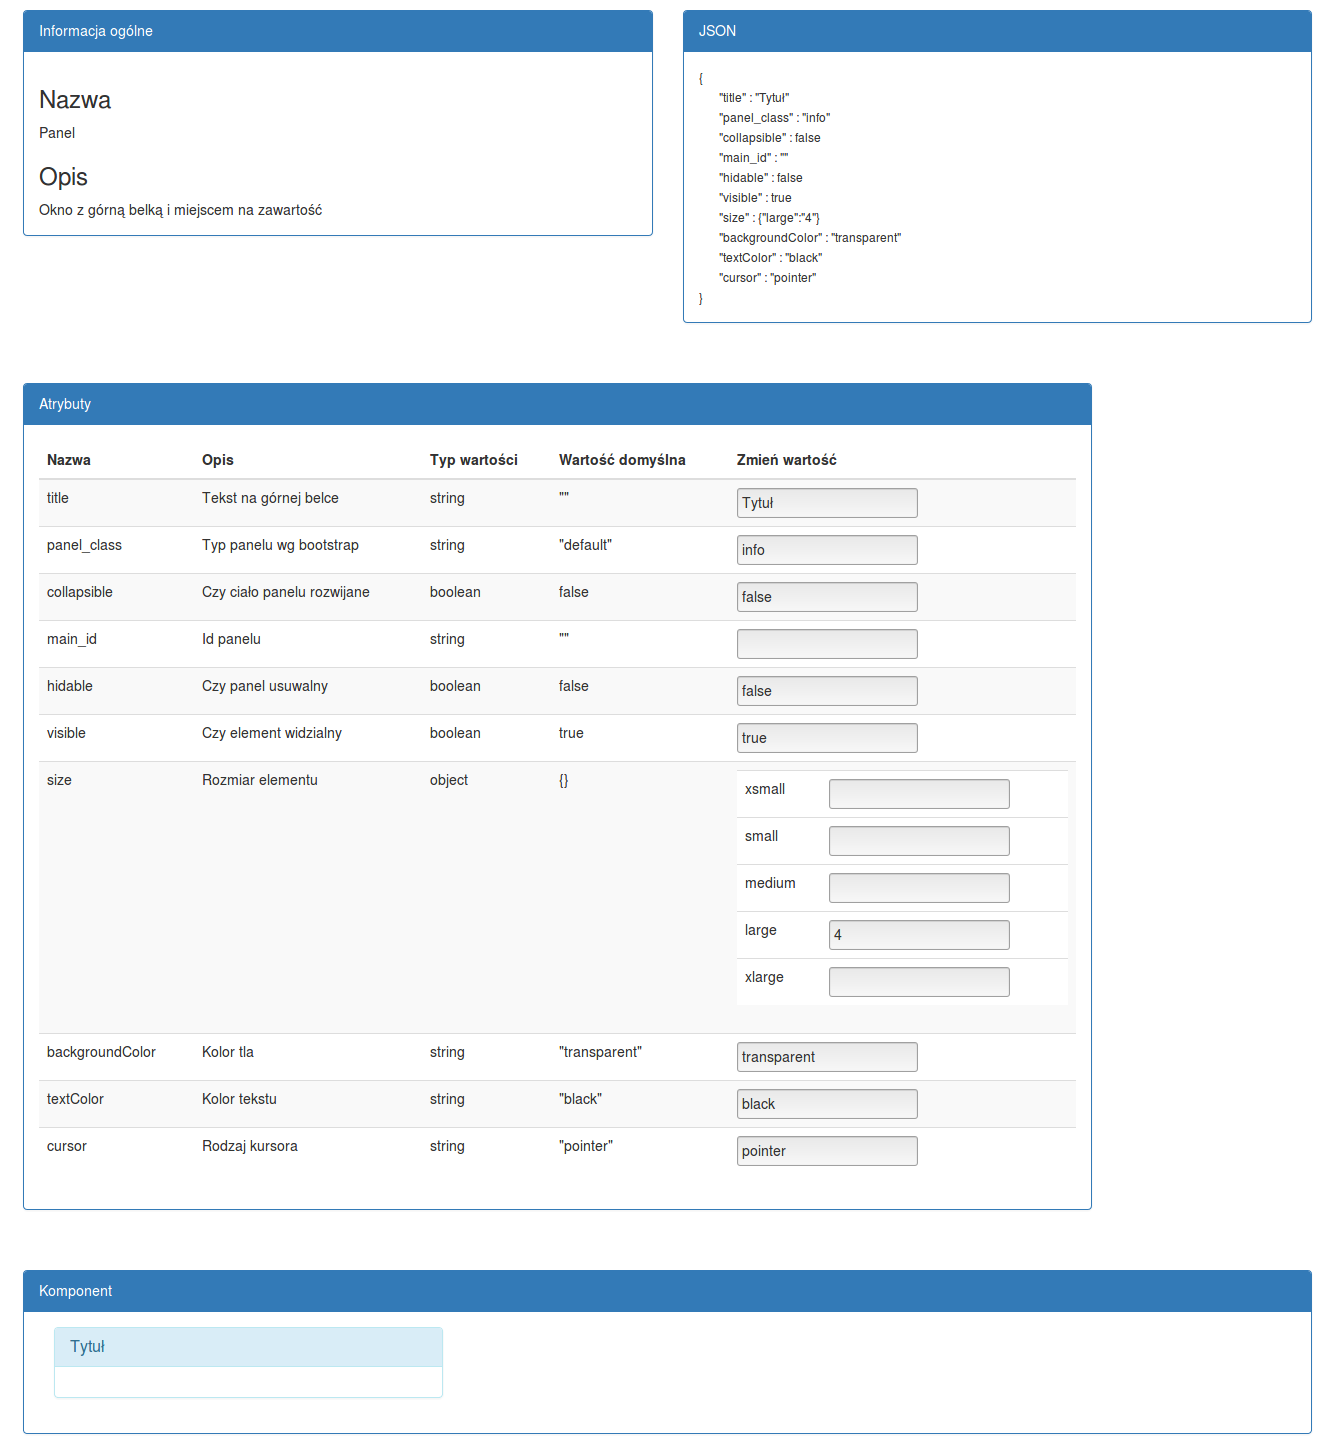
\includegraphics[width=\textwidth]{obrazki/styleguide.png}

\subsection{Interfejs mikrousługi jako JSON}
Na potrzeby realizacji prototypu, pozwoliliśmy sobie na wyspecjalizowanie pewnej grupy mikrousług jako tak zwane mikrousługi formularzowe, to znaczy takie, które pozwalają na skonstruowanie formularza, który wysyła gdzieś dane pobrane od użytkownika.
Do wyświetlenia mikrousługi formularzowej, której interfejs jest opisany obiektem JSON, obiekt ten musi zawierać następujące pola:
\begin{itemize}
	\item $send-url$: adres URL, na który zostanie wysłany formularz
	\item $fill-url$: adres URL, z którego należy pobrać dane dostępnego wypełnienia formularza (dane stałe, np. nazwisko, numer PESEL)
	\item $components$: tablica zawierająca komponenty interfejsu
\end{itemize}
W takiej postaci jest wysyłany na przykład JSON komponentu Plus500.

\subsection{Platforma developera}
Dodawanie nowej mikrousługi do pakietu istniejących jest bardzo proste, chociaż nie udało nam się do końca zaimplementować wszystkich mechanizmów upraszczających. 
W skrócie, wystarczy stworzyć nową klasę języka TypeScript, zaimportować dekorator \mintinline{javascript}{@SetterAlg}, oraz opcjonalnie \mintinline{javascript}{@Register} i \mintinline{javascript}{@Attr} do dokumentacji. 
Następnie wszystkie pola w klasie, które chcemy mieć możliwość ustawiać za pomocą obiektów JSON, dekorujemy \mintinline{javascript}{@SetterAlg} wedle uznania. 
Pozostało jeszcze tylko dodać w funkcji statycznej \mintinline{javascript}{createFromJSON()} mapowanie z żądanej nazwy komponentu w JSONie na instancję klasy (czyli mówiąc prościej, jaką wartością w polu $type$ w JSONie chcemy identyfikować nasz komponent). 
Na sam koniec, w głównym module aplikacji, \mintinline{javascript}{src/app/app.module.ts} dodajemy nasz komponent do tablic $declarations$ oraz $entryComponents$. Nasz nowy komponent jest już gotowy do użycia.

\section{Serwer uwierzytelniania i autoryzacji}

Z uwagi na prototypowy charakter naszej pracy nasz Klient nie przywiązywał większej
wagi do rozwiązania problemu uwierzytelniania i autoryzacji użytkowników. Zdecydowaliśmy
się jednak zaimplementować przykładowy serwer celem ukazania kilku ciekawych
możliwości integratora. Serwer autoryzacji jest napisany w języku Python i wykorzystuje
framework gRPC do udostępniania usług, którymi są: zalogowanie i pobranie tokena
dostępowego, unieważnienie tokena, pobranie identyfikatora i uprawnień użytkownika.
Informacją, która identyfikuje użytkownika jest jednorazowy sesyjny token, który
z punktu widzenia pozostałych usług nie zawiera żadnych użytecznych informacji.
Dzięki temu możliwa jest reimplementacja serwera autoryzacji bez utraty kompatybilności
z pozostałymi częściami systemu. Uprawnienia użytkowników są składowane jako maska
bitowa, w której zapalony bit oznacza posiadanie danego uprawnienia.

\section{Integrator}

Integrator został zrealizowany jako standardowa aplikacja internetowa obsługująca
klientów poprzez protokół HTTP(S). Każda mikrousługa rejestrująca się w integratorze
może poprosić o wystawienie dowolnej liczby tzw. końcówek (ang. \textit{endpoint}).
Końcówka jest jednoznacznie określonym adresem, pod którym serwer usługi udostępnia
swoje zasoby. Wyróżniamy trzy typy końcówek:
\begin{itemize}
	\item View - służy do udostępniania statycznych danych bez bezpośredniego
	udziału usługi, która ją utworzyła. Głównym zastosowaniem tej końcówki jest
	przechowywanie JSONa opisującego interfejs użytkownika po stronie frontendu.
	Integrator umożliwia dynamiczną zmianę zawartości końcówek tego typu, co znacząco
	ułatwia prototypowanie interfejsu użytkownika, gdyż projektant nie musi pisać
	własnej mikrousługi która serwowałaby stosowną treść.
	\item Read - służy do pobierania danych z serwera mikrousługi bez powodowania
	skutków ubocznych. Format przesyłanych informacji zależy od typu komponentu
	proszącego o nie w warstwie frontendu.
	\item Write - służy do wykonywania akcji mających efekt uboczny, np. złożenia
	wniosku.
\end{itemize}
Do jednej końcówki typu Read i Write może być przypisanych dowolnie wiele serwerów
usługi. Integrator dla każdego zapytania losowo wybiera jeden z nich i do niego
kieruje wchodzące zapytanie, a następnie przekazuje odpowiedź z powrotem.

Dzięki współpracy integratora z serwerem uwierzytelniania dostęp do poszczególnych
końcówek może być ograniczony tylko do autoryzowanych użytkowników. Identyfikacja
uprawnionych klientów odbywa się poprzez przekazanie tokenu sesji w parametrze zapytania.

W przypadku końcówek o typie Read i Write możliwe jest przechwytywanie i modyfikacja
przesyłanych danych przy pomocy tzw. haków (ang. \textit{hook}). Haki mogą być
osobno zakładane na każdą końcówkę. Na jednej końcówce może być założonych dowolnie
wiele haków, których kolejność wykonywania zależy od nadanego im priorytetu.
Wyróżniamy dwa typy haków:
\begin{itemize}
	\item In - modyfikują zapytania wchodzące do mikrousługi.
	\item Out - modyfikują wychodzące z mikrousługi odpowiedzi na zapytania.
\end{itemize}

Integrator oferuje dwie metody pobierania listy aktywnych końcówek. Dostępne są
one pod adresami:
\begin{itemize}
	\item /menu - zawiera informację o pierwszej końcówce, która powinna zostać
	wyświetlona po załadowaniu frontendu oraz spis zawartości menu. Menu jest
	personalizowane dla każdego użytkownika osobno i zawiera wpisy tylko o tych
	usługach, do których ma dostęp użytkownik. Na wpis menu składają się stopień
	zagnieżdżenia w strukturze drzewa, wyświetlany tytuł i ikonka oraz końcówka,
	która powinna zostać wyświetlona po kliknięciu danego elementu.
	\item /list - wyświetla dane o wszystkich końcówkach i serwerach mikrousług
	do których dostęp ma obecnie zalogowany użytkownik. Otrzymana lista odzwierciedla
	informacje składowane w bazie danych, co czyni ją przydatną przy poszukiwaniu
	błędów podczas fazy rejestracji mikrousług.
\end{itemize}
W każdym z tych przypadków integrator przysyła odpowiedź w formacie JSON, dzięki
czemu możliwe jest maszynowe jej przetwarzanie (na przykład w edytorze mikrousług).

Konfiguracja integratora przechowywana jest w bazie danych ZooKeeper. Każda
mikrousługa musi podczas uruchamiania dodać do niej swoje wpisy. Takie rozwiązanie
jest świadomym złamaniem zasady mówiącej, że baza danych z której korzysta usługa
nie powinna być bezpośrednio dostępna dla innych mikrousług \cite{microsvc}.
Wynikało ono z unikalnych własności wpisów w ZooKeeperze, które mogą być automatycznie
usuwane po ustaniu pracy serwera mikrousługi, np. na skutek awarii lub utraty
połączenia internetowego. Ponadto poszczególne węzły które składają się na drzewo
przechowujące konfigurację integratora mogą być chronione poprzez mechanizm ACL.
Uznaliśmy, że w naszym prototypie nie ma potrzeby reimplementowania funkcjonalności
zapewnianej przez gotowe komponenty.

Początkowo integrator był implementowany w technologii Play Framework. Niestety
w miarę postępu prac ujawnialiśmy kolejne problemy związane z tym frameworkiem,
począwszy od konfliktu zależności pomiędzy pakietami, poprzez niedziałający tryb
SSL, aż po zawieszanie się serwera. Być może było to spowodowane koniecznością
użycia niestabilnej wersji frameworka. Wymienione kłopoty w połączeniu z niezadowalającym
postępem prac skłoniły nas do przepisania integratora w języku Python. Nowa wersja
nazwana przez nas Integratorem 2 nie posiada wymienionych wyżej wad i została
dogłębnie przetestowana w praktyce.

\section{Mikrousługi}

W trakcie prac nad naszym portalem zaimplementowaliśmy niżej wymienione rodzaje
mikrousług. Ich głównym zadaniem było zilustrowanie interfejsu programisty
wykorzystywanego przy współpracy z integratorem, niekoniecznie zaś implementacja
produkcyjnej funkcjonalności. Naszemu Klientowi zależało bowiem, by integracja
poszczególnych warstw aplikacji była możliwie prosta i osiągalna nawet dla nisko
wykształconych i niedoświadczonych programistów.

\subsection{Powiadomienia}

Powiadomienia są pierwszą zaimplementowaną mikrousługą. Jej zadaniem jest wyświetlenie
liczby rozpatrzonych spraw. Aby dokładniej odzwierciedlić realia panujące w
administracji przy każdym zapytaniu odpowiedź jest losowana. Otrzymane dane
zostają następnie wyświetlone na poniższym ekranie:\\
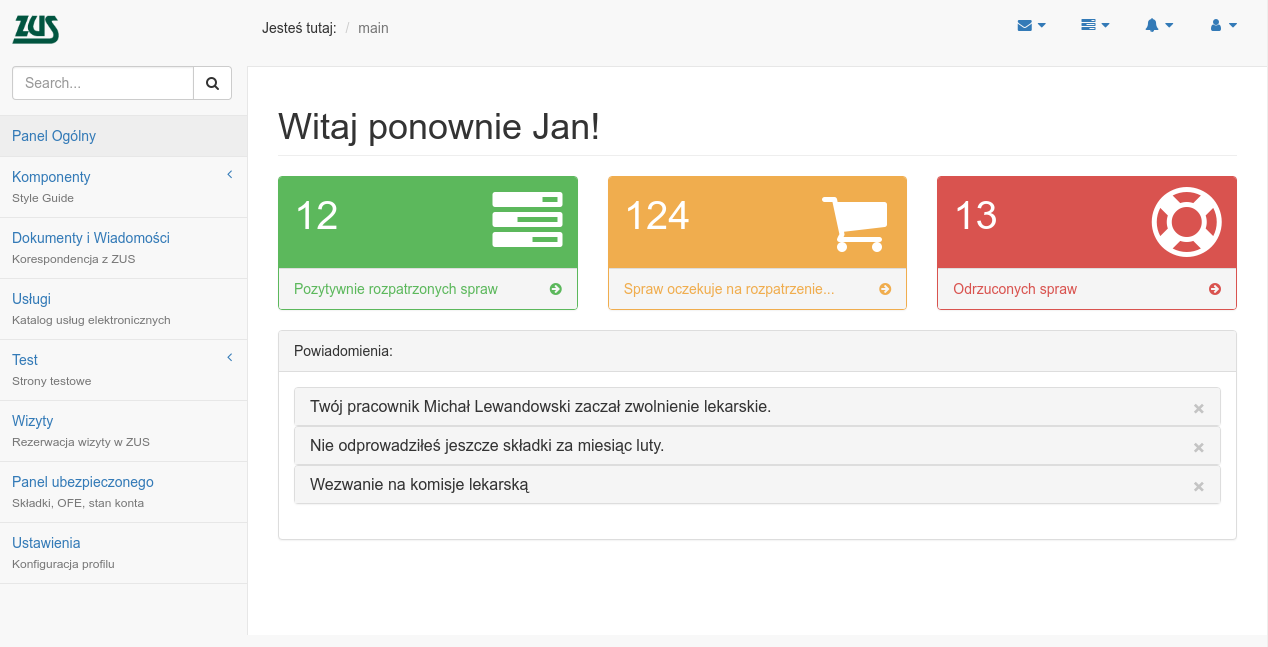
\includegraphics[width=\textwidth]{obrazki/powiadomienia2.png}

Rejestracja usługi odbywa się podczas startu serwera przy użyciu kawałka kodu
analogicznego do poniższego:

\begin{minted}{python}
import notify.installer as inst

addr = "http://localhost:8000"
inst.zk.start()

inst.add_read_endpoint("notify-pending", "server1", addr + "/notify/pending/")
inst.add_write_endpoint("notify-set_variable", "server1", addr +
	"/notify/set_variable/")
\end{minted}
W przedstawionym przykładzie następuje zaimportowanie biblioteki dostarczanej wraz z
integratorem służącej do komunikacji z nim. Następnie zostaje nawiązane połączenie z
serwerem integratora i tworzone są dwie końcówki typu Read i Write o nazwach
,,notify-pending'' i ,,notify-set\_variable'' przypisane do serwera o identyfikatorze
,,server1''. Kiedy integrator zostanie poproszony o dane z końcówki ,,notify-pending'',
wyśle on zapytanie pod adres \texttt{http://localhost:8000/notify/pending/} i przekaże
odpowiedź z powrotem. Wyrejestrowanie usługi z integratora nastąpi automatycznie po
wyłączeniu serwera.

\subsection{Autoryzacja}
Autoryzacja w aplikacjach webowych jest kwestią dosyć skomplikowaną i w naszym prototypie chcieliśmy bardziej przedstawić jakąkolwiek działającą implementację, niż zadbać o jej dopracowanie pod względem bezpieczeństwa.
Domyślne konta w aplikacji to konto $user$, oraz konto $admin$, hasła do kont są domyślnie takie, jak ich nazwy.

\subsection{Logger}

Logger jest mikrousługą ilustrującą działanie mechanizmu haków. Na początku
rejestrowana jest końcówka typu Read o nazwie ,,google'' wraz z odpowiadającym
jej serwerem. Następnie zakładane są haki przy pomocy następujących poleceń:
\begin{minted}{python}
inst.add_node('/hook/in/read/google', '', temp=False)
inst.add_node('/hook/out/read/google', '', temp=False)
inst.add_node('/hook/in/read/google/h1', addr + "/in/", temp=True)
inst.add_node('/hook/out/read/google/h1', addr + "/out/", temp=True)
\end{minted}
Od tej pory cała komunikacja do i z wymienionej końcówki przechodzi przez serwer
mikrousługi, która wykorzystuje ten fakt do wypisywania całego ruchu na konsolę.
Kolejność aplikowania haków zależy od nazwy haka (w tym przypadku ,,h1''), tj.
haki o mniejszych leksykograficznie nazwach są wykonywane wcześniej.

\subsection{Poczta}
Mikrousługa poczty była pierwszą zaimplementowaną usługą, z którą użytkownik
naszej platformy mógł podjąć interakcję. Jak sama nazwa wskazuje, można przy jej
pomocy wysyłać i odbierać wiadomości.\\
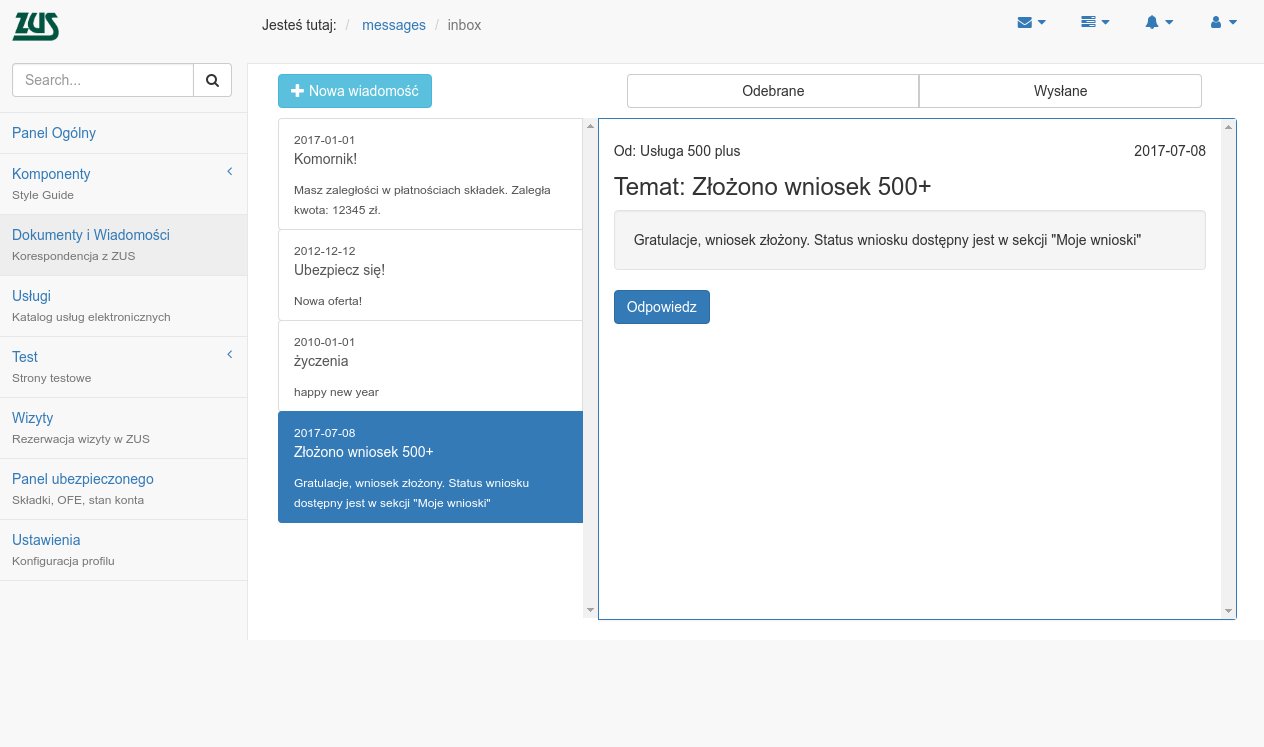
\includegraphics[width=\textwidth]{obrazki/poczta.png}

Tutaj ujawniły się pierwsze mocne strony przyjętej przez nas architektury całego
portalu. Dzięki jasnemu odseparowaniu warstwy prezentacji od warstwy danych
możliwe staje się korzystanie przez mikrousługi z dokładnie tego samego interfejsu,
z którego korzysta warstwa frontendowa portalu do prezentacji danych użytkownikowi.
Przykładowo, kiedy osoba siedząca przed komputerem wysyła wiadomość, to w tej samej
chwili z tej samej końcówki może korzystać aplikacja kliencka na smartfona, system
do zarządzania kadrami, a nawet inna mikrousługa znajdująca się w serwerowni ZUS.
Wykorzystaliśmy ten fakt przy tworzeniu usługi 500+ do wysyłania powiadomień o
udanym złożeniu wniosku.
Unifikacja interfejsów sprawia, że utworzenie, utrzymanie i rozwój mikrousługi jest
tańsze i prostsze. Eliminujemy w ten sposób konieczność utrzymywania kilku redundantnych
kanałów do komunikacji z serwisem oraz w jego obrębie.

\subsection{Plus500}

Z powodu ograniczeń nałożonych na nazwy pakietów w języku Python usługę odpowiedzialną
za obsługę wniosków o świadczenie $500+$ nazwaliśmy ,,Plus500''. Nasza mikrousługa
umożliwia wyświetlenie złożonych wniosków, rozpatrzenie ich przez urzędnika oraz
wysłanie wypełnionego formularza.

Szablon formularza wniosku o świadczenie 500+ plus znajduje się w pliku ,,500plus.form''
i jest opisany w formacie JSON. Po połączeniu z serwerem mikrousługi szablon jest
wysyłany do klienta i wyświetlany. Po naciśnięciu odpowiedniego guzika zawartość
wniosku jest serializowana i wysyłana do mikrousługi.\\
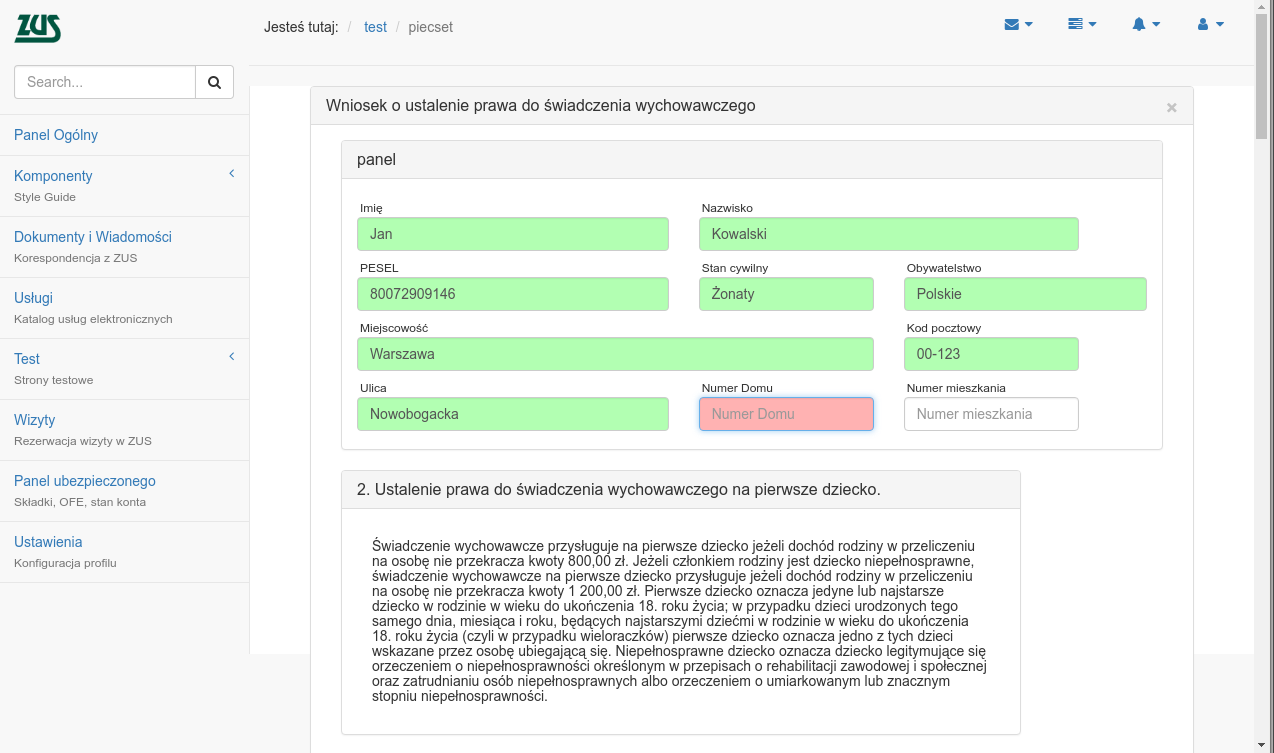
\includegraphics[width=\textwidth]{obrazki/piecset.png}
Rejestracja usługi w integratorze zajmuje tylko 7 linijek kodu:
\begin{minted}{python}
inst.add_view_endpoint_from_file("plus500-wniosek", '500plus.form')
inst.add_read_endpoint("plus500-lista", "server1", addr + "/lista/")
inst.add_read_endpoint("plus500-pokaz", "server1", addr + "/pokaz/")
inst.add_write_endpoint("plus500-send", "server1", addr + "/wyslij/")
inst.add_write_endpoint("plus500-ustaw", "server1", addr + "/ustaw/")
inst.add_menu_element("Moje wnioski 500+", "read/plus500-lista", "/plus500lista")
inst.add_menu_element("Złóż wniosek 500+", "view/plus500-wniosek", "/plus500nowy")
\end{minted}
W powyższym fragmencie widać większość możliwości integratora. Na początku
instalujemy w integratorze plik opisujący formularz o świadczenie 500+. Następnie
dodajemy końcówki które pozwalają na złożenie wniosku i wyświetlenie ich stanu. Na
samym końcu rejestrujemy wpisy w menu. Od tej chwili zmiany są widoczne w interfejsie
użytkownika i możliwa jest interakcja z mikrousługą.

\chapter{Wkład poszczególnych członków zespołu w projekt}

\begin{tabularx}{\linewidth}{|l|X|} \hline
	\textbf{Członek zespołu} & \textbf{Wykonane zadania} \\
	\hline
	Michał Jaroń & Stworzenie architektury warstwy frontend (komponenty). \newline
		      Stworzenie mockupów:
			-> zwolnienie lekarskie
			-> podglądanie kolejek w urzędach
			->
		\newline
		Stworzenie fontendu wiadomości. \newline
		
	\\	
	
	\hline
	Jarosław Socha \newline
		Wyklikanie wniosku 500+ z gotowych komponentów. \newline
		Implementacja front-endu autoryzacji. \newline
		Implementacja komunikacji HTTP z warstwą backend. \newline
		Implementacja renderowania komponentów z obiektów JSON za pomocą dekoratora @SetterAlg. \newline
		Implementacja mechanizmu podglądu i rozpatrywania wniosków.
	\\
	\hline 
	Piotr Zalas & Zaproponowanie wstępnej architektury aplikacji.\newline
	  Implementacja Integratora i Integratora 2.\newline
	  Implementacja mikrousług powiadomień, loggera, poczty, 500+.\newline
	  Implementacja usługi autoryzacji.\newline
	  Implementacja serwera frontendu w Express.js.\newline
	  Przygotowanie diagramów ilustrujących architekturę.\newline
	  Spisanie niniejszej pracy (z wyjątkiem rozdziałów 4.2, 4.3, 6.1 - 6.3).\\
	\hline
\end{tabularx}

\chapter{Podsumowanie}

Jesteśmy usatysfakcjonowani otrzymanym produktem. Udało nam się osiągnąć znaczną
automatyzację procesu zarządzania infrastrukturą. Dzięki automatycznej rejestracji i
wyrejestrowywaniu usług personel techniczny jest zwolniony z wykonywania żmudnej,
powtarzalnej pracy. Zmniejszyliśmy możliwość popełnienia błędu podczas konfiguracji,
a jednocześnie dzięki automatycznemu odcinaniu uszkodzonego serwera od reszty systemu
zwiększyliśmy niezawodność w sposób odczuwalny dla przeciętnego użytkownika.

Zaproponowany przez nas interfejs użytkownika jest wygodny i przyjemny dla oka,
odpowiada najnowszym trendom w projektowaniu witryn internetowych. Spójność interfejsu
została zagwarantowana przez opakowanie jego typowych elementów w system komponentów,
przy projektowaniu którego kierowaliśmy się względami praktycznymi. W pewnych przypadkach
(takich jak okienko wiadomości) bardziej opłacalne było stworzenie jednego dużego
elementu, niż składanie go z kilku mniejszych. Przy tworzeniu formularzy wykorzystaliśmy
wiele małych elementów takich jak pola tekstowe i guziki do stworzenia większej
całości. Separacja danych i warstwy prezentacji pozwala na bezbolesną zmianę wyglądu
portalu bez konieczności jakiejkolwiek ingerencji w elementy pozostałych warstw, w
szczególności mikrousług.

Programiści mikrousług otrzymali od nas narzędzie łączące prostotę tworzenia aplikacji
i dużą siłę wyrazu. Zaproponowany przez nas interfejs pozwala skupić się na tworzeniu
logiki biznesowej z pominięciem niepotrzebnych szczegółów związanych z komunikacją
z innymi częściami systemu oraz dotyczących strony wizualnej. Dzięki rozbiciu
elementów platformy na małe, niezależne części, dalsza rozbudowa i wprowadzanie zmian
w portalu staje się łatwiejsze.

Zastosowanie elastycznej architektury umożliwia dalszy rozwój platformy. Stworzyliśmy
listę rzeczy, które warto w dalszej kolejności zaimplementować i które w znaczący
sposób podniosłyby wartość stworzonego przez nas frameworka. Niestety, ze względu na
ograniczony czas projektu nie byliśmy w stanie ich zaprogramować. Na wymienionej liście
znalazł się miedzy innymi postulat głębszej automatyzacji warstwy frontendu. Obecnie
dodanie nowej usługi wymaga zaangażowania zespołu opiekującego się częścią kliencką
naszego portalu. Chcielibyśmy, żeby mikrousługi miały większy wpływ na jej działanie.
Przykładowo, dodawanie nowych elementów do menu głównego mogłoby się odbywać w pełni
automatycznie. Mikrousługa mogłaby też mieć możliwość zapisywania i odczytywania danych
w kliencie, a także wskazywania końcówki która ma być wyświetlona jako następna.
Dzięki temu możliwe stałoby się konstruowanie wielostronnicowych formularzy, które
krok po kroku prowadziłyby użytkownika przez proces wypełniania wniosku.

Usprawnienia są możliwe także po stronie backendu. Do najprostrzych może należeć
automatyczne wykrywanie serwera integratora na zasadzie podobnej do stosowanej
w protokole DHCP. Obecnie trzeba jawnie podawać adres integratora, co w dynamicznie
zmieniającym się środowisku nie powinno mieć miejsca. Bardziej złożonymi problemami
zarysowanymi już w rozdziale 3 jest orchestracja mikrousług i uspójnianie między
nimi danych w przypadku konfliktu. Problem orchestracji może być częściowo
rozwiązany poprzez mechanizm haków, który umożliwia tworzenie operacji obejmujących
wiele usług, jednak naszym zdaniem jest to rozwiązanie dalekie od optymalnego.

Powyższa lista powstała na wyraźne życzenie naszego Klienta, który był zainteresowany
perspektywami dalszego rozwoju stworzonego przez nas prototypu. Niewątpliwie tematyka
mikrousług i architektury zorientowanej na usługi jeszcze nie raz będzie przedmiotem
naszego zawodowego zainteresowania. Jako zespół mamy wielką nadzieję, że spełniliśmy
pokładane w nas oczekiwania.

\appendix
\chapter{Spis zawartości dołączonej płyty CD}
Dołączona do pracy płyta zawiera następujące pliki i katalogi:

\section{Katalog \mintinline{python}{/backend/}}
TODO

\section{Katalog \mintinline{python}{/frontend/}}
TODO

\section{Plik \mintinline{python}{Instalacja - Backend.pdf}}
Instrukcja instalacji i uruchomienia części backendowej naszej aplikacji

\section{Plik \mintinline{python}{Instalacja - Frontend.pdf}}
Instrukcja instalacji i uruchomienia części frontendowej naszej aplikacji

\section{Katalog \mintinline{python}{/prezentacja/}}
Prezentacja z dnia 10.06.2017

\section{Plik \mintinline{python}{README}}
Plik zawierający dodatkowe informacje na temat zawartości płyty

%Dokładny spis zawartości towarzyszącej płytki (p. dalej). To bardzo ważne, proszę zapisać jako osobny rozdział (czyli np. nie podrozdział). Płytka CD/DVD/Blu-ray/...
%
%Zawiera:\\
%Pełną dokumentacją projektu w łatwo dającym się odczytać formacie (najlepiej pdf + źródło).
%Program (w postaci źródłowej i potencjalnie umożliwiającej uruchomienie, to może oznaczać np. dostarczenie stosownych plików makefile, pomocniczych plików z danymi, opisu instalacji itp.).
%Wszelkie inne dokumenty powstałe podczas zajęć (np. teksty prezentacji, teksty pracy z poprzedniego dużego punktu, itp.).
%
%Płyta jest częścią pracy - trzeba tyle płyt co drukowanych egzemplarzy pracy. Płytkę trzeba przymocować do pracy, tak by a) nie wypadała b) dało się ją wyjąć i odczytać w komputerze :).


%\chapter{Zrzuty ekranu z naszej aplikacji}
% TODO

%\chapter{Obserwator emerytalny}
%Z uwagi na bardzo niepewny charakter naszego projektu i trudności związane z
%formalnym rozliczeniem naszej pracy zdecydowaliśmy się wykonać niejako poza
%głównym projektem serwis ,,Obserwator emerytalny''.

\begin{thebibliography}{99}
\addcontentsline{toc}{chapter}{Bibliografia}

\bibitem[1]{curator} Apache, \textit{Apache Curator},
http://curator.apache.org/. [Dostęp: 2017-06-22].

\bibitem[2]{curatorlock} Apache, \textit{Apache Curator - Shared Lock},
http://curator.apache.org/curator-recipes/shared-lock.html. [Dostęp: 2017-06-22].

\bibitem[3]{distibutedlog} Apache, \textit{DistributedLog},
http://distributedlog.incubator.apache.org/. [Dostęp: 2017-06-22].

\bibitem[4]{kafka} Apache, \textit{Kafka},
https://kafka.apache.org/. [Dostęp: 2017-06-22].

\bibitem[5]{zookeeper} Apache, \textit{Apache ZooKeeper},
https://zookeeper.apache.org/. [Dostęp: 2017-06-22].

\bibitem[6]{microsvc} Chris Richardson, \textit{Microservice architecture patterns and best practices},
http://microservices.io/. [Dostęp: 2017-06-22].

\bibitem[7]{redislock} \textit{Distributed locks with Redis},
https://redis.io/topics/distlock. [Dostęp: 2017-06-22].

\bibitem[8]{django} Django Software Foundation, \textit{Django},
https://www.djangoproject.com/. [Dostęp: 2017-06-22].

\bibitem[9]{react} Facebook, \textit{React},
https://facebook.github.io/react/. [Dostęp: 2017-06-22].

\bibitem[10]{angular2} Google, \textit{Angular},
https://angular.io/. [Dostęp: 2017-06-22].

\bibitem[11]{grpc} Google, \textit{gRPC},
http://www.grpc.io/. [Dostęp: 2017-06-22].

\bibitem[12]{govsm} \textit{Government Service Design Manual},
https://www.gov.uk/service-manual/index.html. [Dostęp: 2017-06-22].

\bibitem[13]{fowlermicroservices} James Lewis, Martin Fowler, \textit{Microservices},
https://martinfowler.com/articles/microservices.html. [Dostęp: 2017-06-22].

\bibitem[14]{kazoo} Kazoo team, \textit{Kazoo},
https://github.com/python-zk/kazoo. [Dostęp: 2017-06-22].

\bibitem[15]{beanstalkd} Keith Rarick, \textit{Beanstalkd},
http://kr.github.io//beanstalkd/. [Dostęp: 2017-06-22].

\bibitem[16]{play} Lightbend, \textit{Play Framework},
https://www.playframework.com/. [Dostęp: 2017-06-22].

\bibitem[17]{redisbad} Martin Kleppmann, \textit{How to do distributed locking},
http://martin.kleppmann.com/2016/02/08/how-to-do-distributed-locking.html. [Dostęp: 2017-06-22].

\bibitem[18]{mcobywatel} Ministerstwo Cyfryzacji, \textit{Portal Rzeczypospolitej Polskiej - Opis projektu},
https://mc.gov.pl/projekty/portal-rzeczypospolitej-polskiej/opis-projektu. [Dostęp: 2017-06-22].

\bibitem[19]{expressjs} Node.js Foundation, \textit{Express},
https://expressjs.com/. [Dostęp: 2017-06-22].

\bibitem[20]{hauer} Philipp Hauer, \textit{Microservices in a Nutshell. Pros and Cons.},
https://blog.philipphauer.de/microservices-nutshell-pros-cons/. [Dostęp: 2017-06-22].

\bibitem[21]{reactlicense} React, etc. Tech Stack, \textit{Your license to use React.js can be revoked if you compete with Facebook},
http://react-etc.net/entry/your-license-to-use-react-js-can-be-revoked-if-you-compete-with-facebook. [Dostęp: 2017-06-22].

\bibitem[22]{redisson} \textit{Redisson},
http://redisson.org/. [Dostęp: 2017-06-22].

\bibitem[23]{mammatustech} Rick Hightower, \textit{Java Microservices Architecture},
http://www.mammatustech.com/java-microservices-architecture. [Dostęp: 2017-06-22].

\bibitem[24]{sqlite} SQLite Consortium, \textit{SQLite},
https://www.sqlite.org/. [Dostęp: 2017-06-22].

\bibitem[25]{postgres} The PostgreSQL Global Development Group, \textit{PostgreSQL},
https://www.postgresql.org/. [Dostęp: 2017-06-22].

\bibitem[26]{tfa} \textit{The Twelve-Factor App}, https://12factor.net/. [Dostęp: 2017-06-22].

\bibitem[27]{nginx} Tony Mauro, \textit{Adopting Microservices at Netflix: Lessons for Architectural Design},
https://www.nginx.com/blog/microservices-at-netflix-architectural-best-practices/. [Dostęp: 2017-06-22].

\bibitem[28]{bootstrap} Twitter, \textit{Bootstrap},
http://getbootstrap.com/. [Dostęp: 2017-06-22].

\bibitem[29]{wsdl} World Wide Web Consortium, \textit{Web Services Description Language},
https://www.w3.org/TR/wsdl. [Dostęp: 2017-06-22].

\bibitem[30]{zuspue} ZUS, \textit{Platforma Usług Elektronicznych},
http://pue.zus.pl/. [Dostęp: 2017-06-22].

\bibitem[31]{rocznik} ZUS, \textit{Rocznik Statystyczny Ubezpieczeń Społecznych},
http://www.zus.pl/baza-wiedzy/statystyka/rocznik-statystyczny-ubezpieczen-spolecznych. [Dostęp: 2017-06-22].

\end{thebibliography}

\end{document}
